\documentclass[journal]{vgtc}        % final (journal style)
%\documentclass[review,journal]{vgtc}         % review (journal style)
%\documentclass[widereview]{vgtc}             % wide-spaced review
%\documentclass[preprint,journal]{vgtc}       % preprint (journal style)

%% Uncomment one of the lines above depending on where your paper is
%% in the conference process. ``review'' and ``widereview'' are for review
%% submission, ``preprint'' is for pre-publication, and the final version
%% doesn't use a specific qualifier.

%% Please use one of the ``review'' options in combination with the
%% assigned online id (see below) ONLY if your paper uses a double blind
%% review process. Some conferences, like IEEE Vis and InfoVis, have NOT
%% in the past.

%% Please note that the use of figures other than the optional teaser is not permitted on the first page
%% of the journal version.  Figures should begin on the second page and be
%% in CMYK or Grey scale format, otherwise, colour shifting may occur
%% during the printing process.  Papers submitted with figures other than the optional teaser on the
%% first page will be refused. Also, the teaser figure should only have the
%% width of the abstract as the template enforces it.

%% These few lines make a distinction between latex and pdflatex calls and they
%% bring in essential packages for graphics and font handling.
%% Note that due to the \DeclareGraphicsExtensions{} call it is no longer necessary
%% to provide the the path and extension of a graphics file:
%% 
\includegraphics{diamondrule} is completely sufficient.
%%
\ifpdf%                                % if we use pdflatex
  \pdfoutput=1\relax                   % create PDFs from pdfLaTeX
  \pdfcompresslevel=9                  % PDF Compression
  \pdfoptionpdfminorversion=7          % create PDF 1.7
  \ExecuteOptions{pdftex}
  \usepackage{graphicx}                % allow us to embed graphics files
  \DeclareGraphicsExtensions{.pdf,.png,.jpg,.jpeg} % for pdflatex we expect .pdf, .png, or .jpg files
\else%                                 % else we use pure latex
  \ExecuteOptions{dvips}
  \usepackage{graphicx}                % allow us to embed graphics files
  \DeclareGraphicsExtensions{.eps}     % for pure latex we expect eps files
\fi%

%% it is recomended to use ``\autoref{sec:bla}'' instead of ``Fig.~\ref{sec:bla}''
\graphicspath{{gfx/}{./}} % where to search for the images

\usepackage{microtype}                 % use micro-typography (slightly more compact, better to read)
\PassOptionsToPackage{warn}{textcomp}  % to address font issues with \textrightarrow
\usepackage{textcomp}                  % use better special symbols
\usepackage{mathptmx}                  % use matching math font
\usepackage{times}                     % we use Times as the main font
\renewcommand*\ttdefault{txtt}         % a nicer typewriter font
\usepackage{cite}                      % needed to automatically sort the references
\usepackage{tabu}                      % only used for the table example
\usepackage{booktabs}                  % only used for the table example
\usepackage{makecell}
\usepackage{multirow}
\usepackage[export]{adjustbox}
\usepackage{subfig}
\usepackage{enumitem}

\usepackage{xcolor}
\newcommand{\tnote}[3]{{\color{#2}#1: #3}}
%\newcommand{\change}[1]{\textcolor{red}{#1}}
%\newcommand{\removed}[1]{\textcolor{red}{\sout{#1}}}
% \newcommand{\change}[1]{{\color{red}#1}}
\newcommand{\change}[1]{{#1}}


\newcommand{\removed}[1]{}
\newcommand{\DaH}[1]{\tnote{DaH}{red}{#1}}
\newcommand{\HP}[1]{\tnote{HP}{green}{#1}}
\newcommand{\JT}[1]{\tnote{JT}{blue}{#1}}
\newcommand{\IGNORE}[1]{}

%% We encourage the use of mathptmx for consistent usage of times font
%% throughout the proceedings. However, if you encounter conflicts
%% with other math-related packages, you may want to disable it.

%% In preprint mode you may define your own headline.
%\preprinttext{To appear in IEEE Transactions on Visualization and Computer Graphics.}

%% If you are submitting a paper to a conference for review with a double
%% blind reviewing process, please replace the value ``0'' below with your
%% OnlineID. Otherwise, you may safely leave it at ``0''.
\onlineid{0}

%% declare the category of your paper, only shown in review mode
\vgtccategory{Research}
%% please declare the paper type of your paper to help reviewers, only shown in review mode
%% choices:
%% * algorithm/technique
%% * application/design study
%% * evaluation
%% * system
%% * theory/model
\vgtcpapertype{theory/model}

%% Paper title.
% James' title suggestions
% - Reproducing 'Graphical Perception' with CNNs
% - 
\title{Supplemental Material for\\Evaluating `Graphical Perception' with CNNs}

%% This is how authors are specified in the journal style

%% indicate IEEE Member or Student Member in form indicated below
%\author{Daniel Haehn, \textit{Member, IEEE}, James Tompkin, and Hanspeter Pfister}
\author{Daniel Haehn, James Tompkin, and Hanspeter Pfister}
\authorfooter{
%% insert punctuation at end of each item
\item Daniel Haehn, and Hanspeter Pfister are with Harvard University. \\
E-mail: \{haehn,pfister\}@seas.harvard.edu.
%
\item James Tompkin is with Brown University. \\E-mail: james\_tompkin@brown.edu.
}

%other entries to be set up for journal
\shortauthortitle{Haehn \MakeLowercase{\textit{et al.}}: Evaluating `Graphical Perception' with CNNs}
%\shortauthortitle{Firstauthor \MakeLowercase{\textit{et al.}}: Paper Title}


%% ACM Computing Classification System (CCS). 
%% See <http://www.acm.org/class/1998/> for details.
%% The ``\CCScat'' command takes four arguments.

%\CCScatlist{ % not used in journal version
% \CCScat{K.6.1}{Management of Computing and Information Systems}%
%{Project and People Management}{Life Cycle};
% \CCScat{K.7.m}{The Computing Profession}{Miscellaneous}{Ethics}
%}

%% Uncomment below to include a teaser figure.
%\teaser{
%  \centering
%\par{\\~\\~\\~\\}
%}

%% Uncomment below to disable the manuscript note
\renewcommand{\manuscriptnotetxt}{}

%% Copyright space is enabled by default as required by guidelines.
%% It is disabled by the 'review' option or via the following command:
% \nocopyrightspace

%\vgtcinsertpkg

%%%%%%%%%%%%%%%%%%%%%%%%%%%%%%%%%%%%%%%%%%%%%%%%%%%%%%%%%%%%%%%%
%%%%%%%%%%%%%%%%%%%%%% START OF THE PAPER %%%%%%%%%%%%%%%%%%%%%%
%%%%%%%%%%%%%%%%%%%%%%%%%%%%%%%%%%%%%%%%%%%%%%%%%%%%%%%%%%%%%%%%%

\begin{document}
\maketitle
%% The ``\maketitle'' command must be the first command after the
%% ``\begin{document}'' command. It prepares and prints the title block.

%% the only exception to this rule is the \firstsection command

\section{Additional Experiments}

\subsection{Anti-aliasing}
One way to increase the fidelity of the information given to the network for angled or curved lines is to anti-alias the line drawing. This provides grayscale intensity values to smooth out the jagged line edges and may be more suitable to networks trained on natural images (such as VGG19~* and Xception~*, with ImageNet weights).

We conduct an experiment to measure continuous pie chart angles from stimuli with anti-aliased (AA) lines (Figure~\ref{fig:aa}). There is a slight increase in performance for the AA case for VGG19 *, and an even slighter increase for Xception *. However, overall, adding anti-aliasing to the line generation was not statistically significant to the tested CNNs when comparing the performance across all networks ($F(1,30)=0.341, p>0.5$). This is not surprising since smoothing only changes very little information at the resolution of our stimuli. Smooth edges might add more value on higher-resolution stimuli. % which we plan to evaluate in the future.

%\JT{Where is the comparison to the `from scratch' stimuli? Can we say anything about this here?} \JT{What statistical test is this? Is it across all conditions, or just for VGG19? YES this is across all conditions... whether the average result changes}

% In our experiments, we chose to create visualizations without interpolation, and to estimate integer-valued measurements.

\begin{figure}[p]
\centering
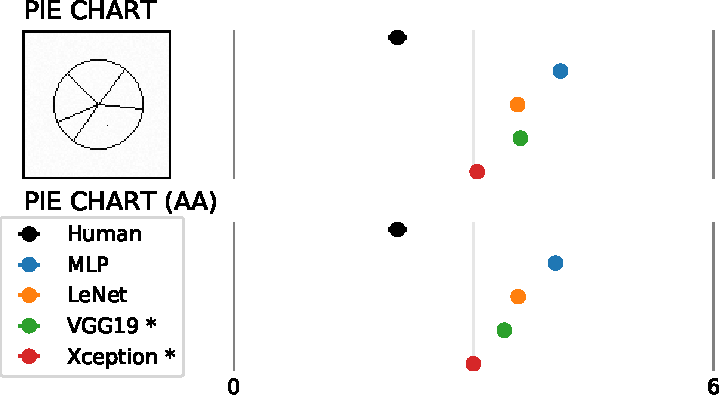
\includegraphics[width=.825\linewidth]{../gfx/figure3_mlae_better_all_AA.pdf}
\caption{\textbf{Anti-aliasing.} We test whether anti-aliasing affects the performance of our networks on pie charts by measuring MLAE. Starred networks are fine-tuned from ImageNet weights. The difference is not statistically significant ($F(1,30)=0.341,p>0.5$).}
\label{fig:aa}
\end{figure}

\subsection{Noise}

For all our experiments, we add subtle $5\%$ noise to every pixel to enhance variability. We did not observe a significant effect on regression performance when comparing the Weber-Fechner's law experiment with and without noise, averaged over 4 runs (Figure~\ref{fig:noise}). However, the variability of LeNet increased with the additional complexity.

\begin{figure}[p]
\centering
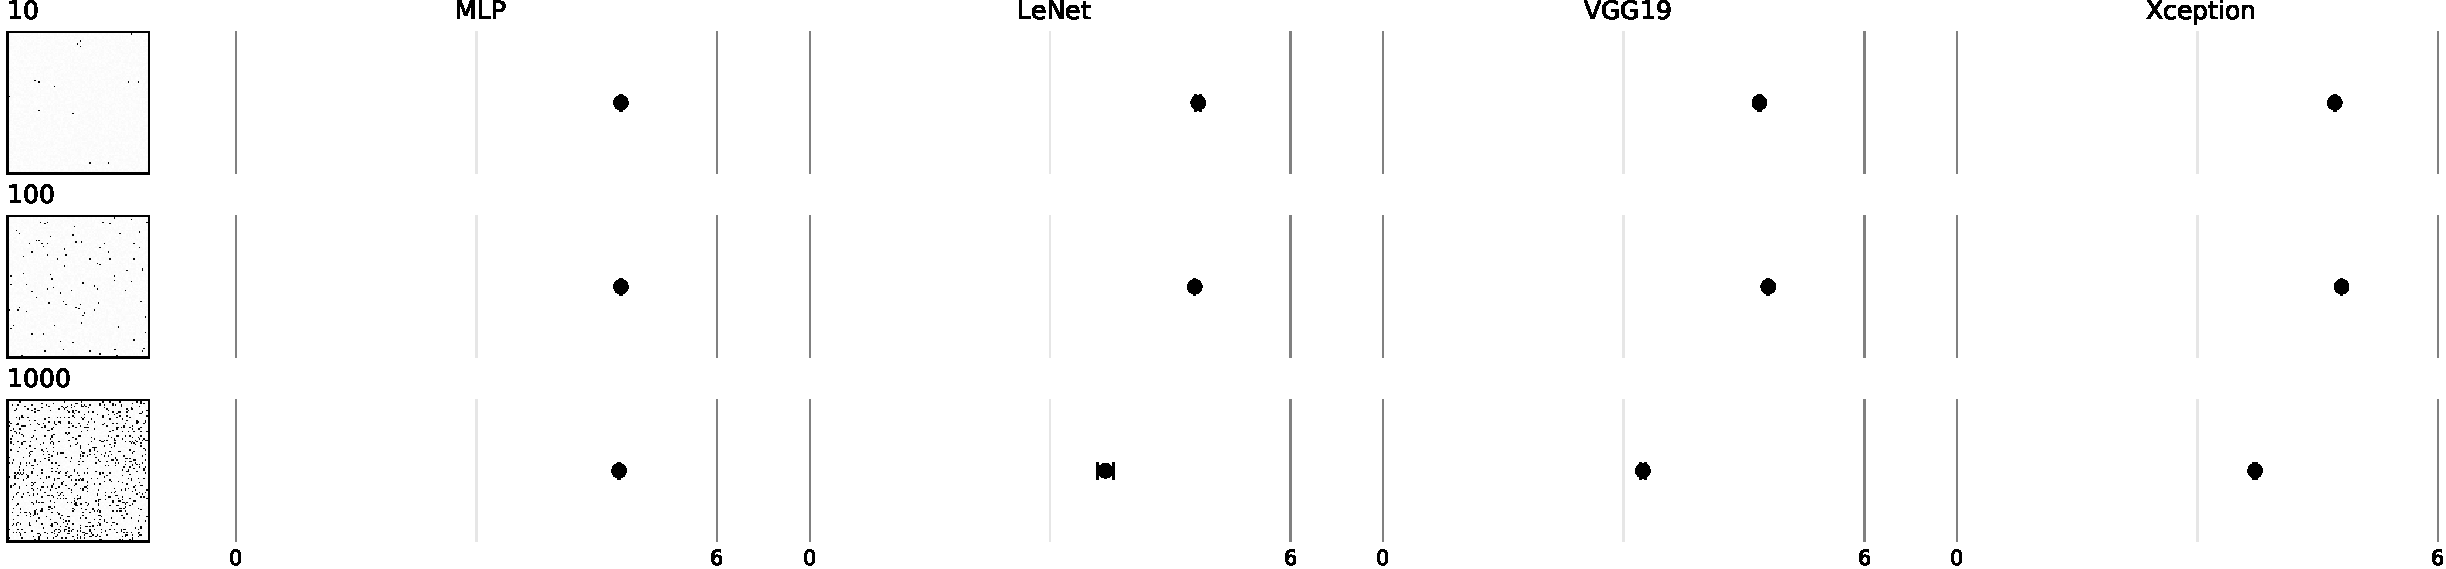
\includegraphics[width=.825\linewidth]{../gfx/weber_mlae_no_noise.pdf}\\
\vspace{0.4cm}
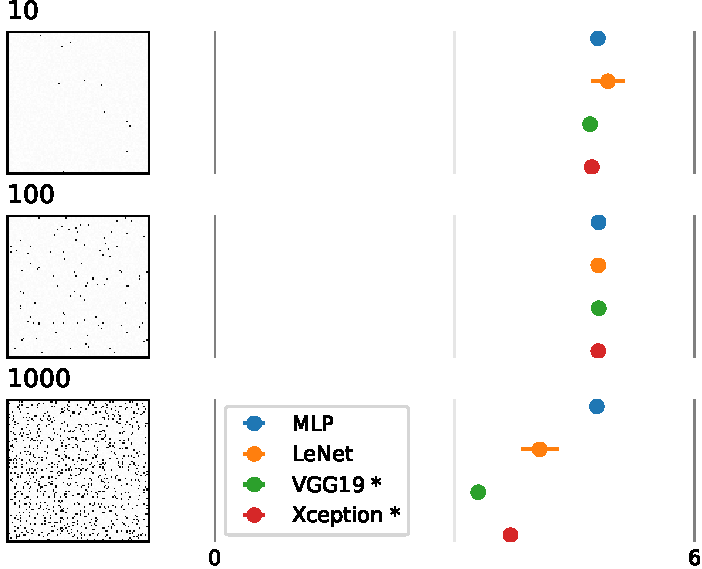
\includegraphics[width=.825\linewidth]{../gfx/weber_mlae_noise.pdf}
\caption{\textbf{Noise.} We test whether noise affects the performance of our networks on the Weber-Fechner's law experiment by measuring MLAE. \emph{Top:} With noise, $MLAE=4.511$ ($SD=0.512$). \emph{Bottom:} Without noise $MLAE=4.491$ ($SD=0.543$). The difference is not statistically significant ($F(1,22)=0.008,p>0.5$).}
\label{fig:noise}
\end{figure}

\section{Comparisons to Cleveland and McGill's Stimuli}

\change{
We visually compare our stimuli to those of Cleveland and McGill~\cite{cleveland_mcgill}, and explain our choices for any differences.
}

\subsection{Resolution Differences}

\change{
Cleveland and McGill's stimuli were created on 8.5$\times$11 inch paper and presented to participants in a binder. While it is unclear from their paper how the stimuli were created (e.g., printed from a digital file, or drawn with pen), it is safe to assume that there is a resolution difference from our stimuli. Our stimuli are 100$\times$100 digital images, with their resolution chosen for computational reasons: We needed to train more than 2,500 models and, at this resolution, our most complex Xception model took 6 hours to train with 60,000 stimuli.

This limited resolution affects network performance in making precise estimates, especially in tasks that require estimating lines drawn at angles or curved lines. As we draw binary stimuli, there are only so many angles of lines that can be drawn within 100$\times$100 pixels that produce different visual output. This leads to a performance floor or constant error. For instance, on average, we can only draw binary angled lines with 1.45 degrees of accuracy (0.67 standard deviation).

% Point about input size, layers, receptive fields, etc.?
}

%%%%%%%%%%%%%%%%%%%%%%%%%%%%%%%%%%%%%%%%%%%%%%%%%
% Pre-declaring some figures for good placement %
%%%%%%%%%%%%%%%%%%%%%%%%%%%%%%%%%%%%%%%%%%%%%%%%%


\begin{figure*}[tb]
    \centering
    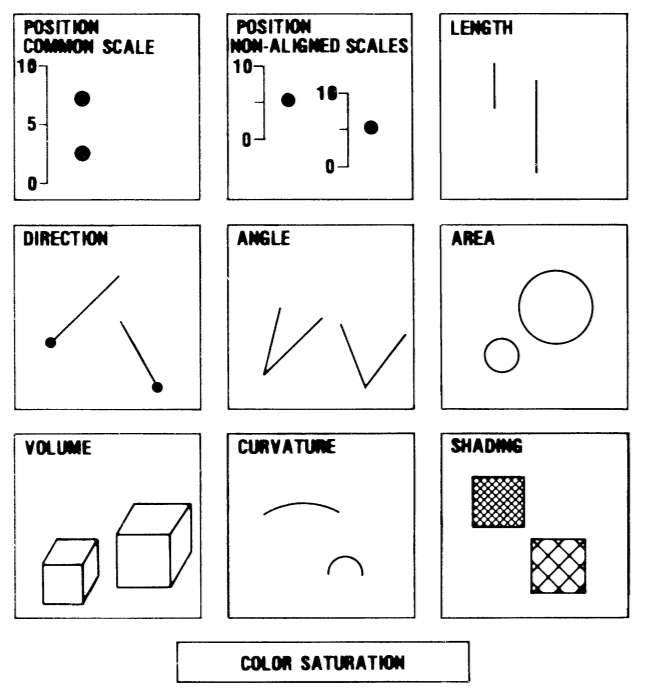
\includegraphics[width=0.49\linewidth]{./gfx/CMcG_Comparison/CMcG_ElementaryPerceptualTasks.png}
    \vrule
    \hspace{0.2cm}
    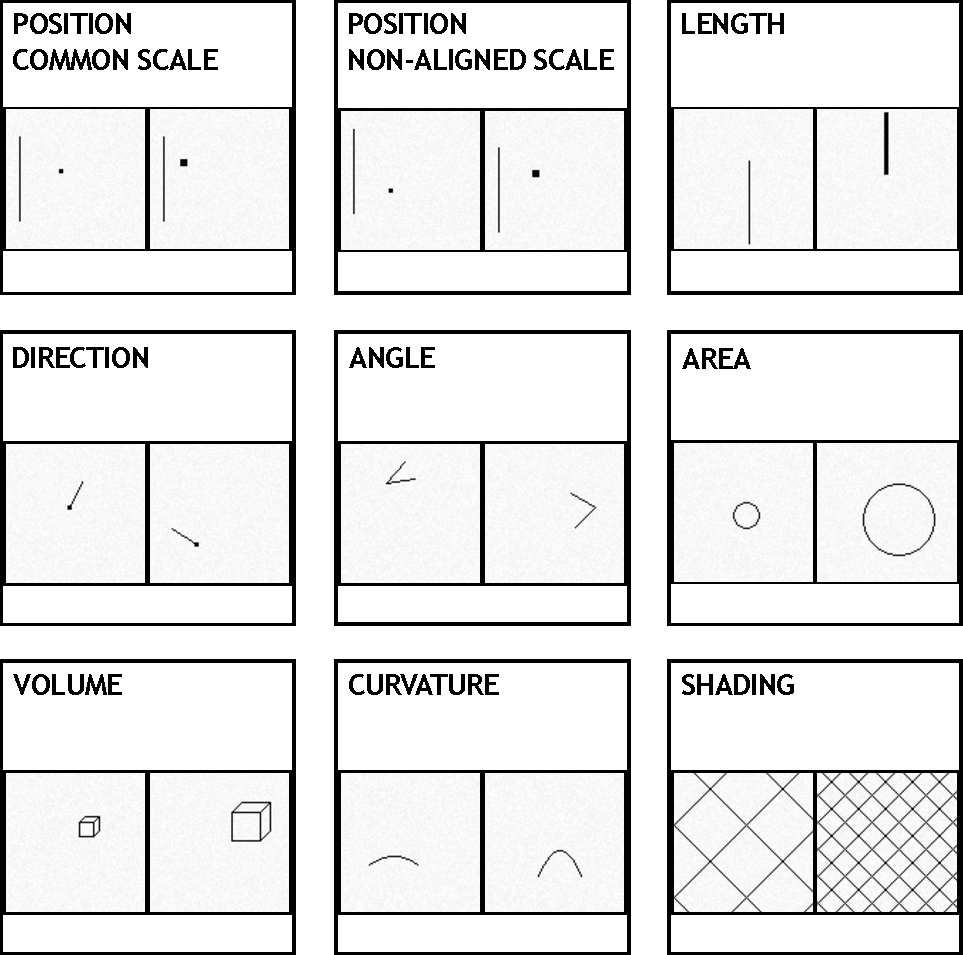
\includegraphics[width=0.465\linewidth,trim=0 -2.00cm 0 0, clip]{./gfx/CMcG_Comparison/Ours_ElementaryPerceptualTasks.pdf}
    \caption{\emph{Left:} Cleveland and McGill's example figure for their elementary perceptual tasks, with each task showing variation through two sample examples (Figure 1 from \cite{cleveland_mcgill}). \emph{Right:} Two example stimuli from our elementary perceptual task experiment. Note that the border around each of our stimuli only exist in this figure to visually separate the stimuli; no border exists in our experiments. Our stimuli also include minor variations in style, such as dot and stroke width in position and length. Finally, as per Cleveland and McGill, we defer color saturation as a perceptual problem for future work. (Though given the success of CNNs in estimating elementary graphical perception task values in comparison to humans, we would also expect CNNs to be more successful than humans at estimating color saturation.)}
    \label{fig:cmcg_elementary_comparison}
\end{figure*}




\subsection{Elementary Perceptual Tasks}

\change{
Cleveland and McGill provide an explanatory figure for their defined elementary perceptual tasks, with each example showing the expected variation in parameter through two samples. We compare visually to two samples of our stimuli (Figure \ref{fig:cmcg_elementary_comparison}). Our stimuli are similar in appearance, with the addition that our stimuli also include minor variations in style such as dot and stroke width in position and length.

One difference is that we exclude the numerical values written as text along the scale in the `Position Common Scale' and `Position Non-aligned Scales' examples. While training a CNN to recognize text on graphs is possible given enough examples~\cite{kafle2018dvqa}, in our case these numbers would not change from stimuli to stimuli and so the network would not gain any information between stimuli to help solve the position estimation problem. As such, we simplify the task by removing the redundant numbers, with the scale values implicitly encoded by the size of the image and the location of the line start and end pixels.

By the same reasoning, the scale itself is redundant in the `Position Common Scale' task as it does not move---the network must map the vertical pixel positions of the dots to the quantity range of numbers. We keep the scale to allow comparison with the `Position Non-aligned Scale' task. Further, when we train networks that look at \emph{all} elementary perceptual tasks, keeping the scale allows the network to exploit the consistency of representation across the two position estimation tasks.
}

Finally, we list the permutations of each stimuli in Table \ref{tab:encoding_parameters}.


\begin{table}[t]
\centering
\caption{\textbf{Elementary Perceptual Tasks.} Rasterized visualizations of our elementary perceptual tasks as defined by Cleveland and McGill~\cite{cleveland_mcgill} (color saturation excluded). We sequentially increase the number of parameters for every task (e.g., by adding translation). This introduces variability and creates increasingly more complex datasets.}
\resizebox{0.9\linewidth}{!}{
\begin{tabular}{lllr}
	\toprule
	\multicolumn{2}{l}{Elementary Perceptual Task} & ~ & Permutations\\
	\midrule
	\raisebox{-.85\height}{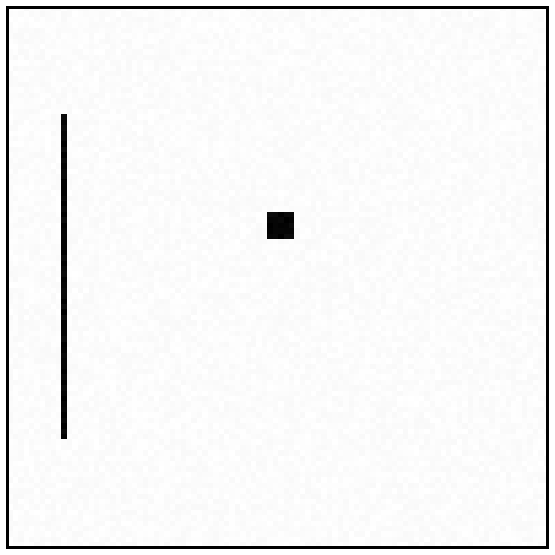
\includegraphics[width=.5in]{../gfx/position_common_scale.pdf}} & \makecell[tl]{\emph{Position Common Scale}\\~~~Position Y\\~~~+ Position X \\~~~+ Spot Size \\} &~& \makecell[tr]{~\\ $60$ \\ $3,600$ \\ $21,600$}\\

	\midrule
	\raisebox{-.85\height}{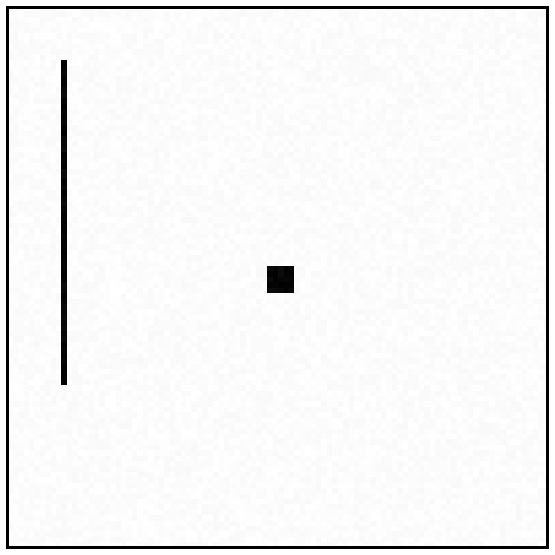
\includegraphics[width=.5in]{../gfx/position_non_aligned_scale.pdf}} & \makecell[tl]{\emph{Position Non-Aligned Scale}\\~~~Position Y\\~~~+ Position X \\~~~+ Spot Size \\} &~& \makecell[tr]{~\\ $600$ \\ $36,000$ \\ $216,000$}\\

	\midrule
	\raisebox{-.95\height}{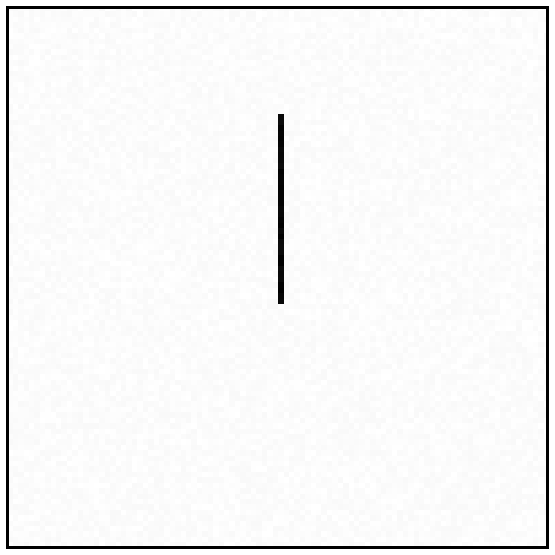
\includegraphics[width=.5in]{../gfx/length.pdf}} & \makecell[tl]{\emph{Length}\\~~~Length\\~~~+ Position Y \\~~~+ Position X \\~~~+ Width} &~& \makecell[tr]{ ~\\$60$ \\ $2,400$ \\ $144,000$\\$864,000$}\\

	\midrule
	\raisebox{-.85\height}{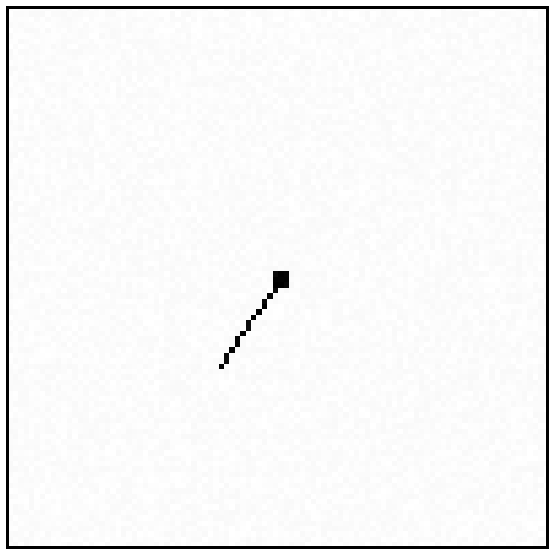
\includegraphics[width=.5in]{../gfx/direction.pdf}} & \makecell[tl]{\emph{Direction}\\~~~Angle\\~~~+ Position Y \\~~~+ Position X} &~& \makecell[tr]{ ~\\$360$ \\ $21,600$ \\ $1,296,000$}\\

	\midrule
	\raisebox{-.85\height}{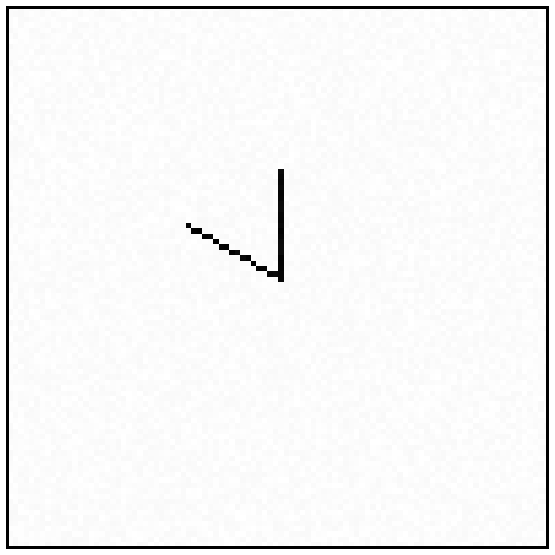
\includegraphics[width=.5in]{../gfx/angle.pdf}} & \makecell[tl]{\emph{Angle}\\~~~Angle\\~~~+ Position Y \\~~~+ Position X} &~& \makecell[tr]{ ~\\$90$ \\ $5,400$ \\ $324,000$}\\

	\midrule
	\raisebox{-.85\height}{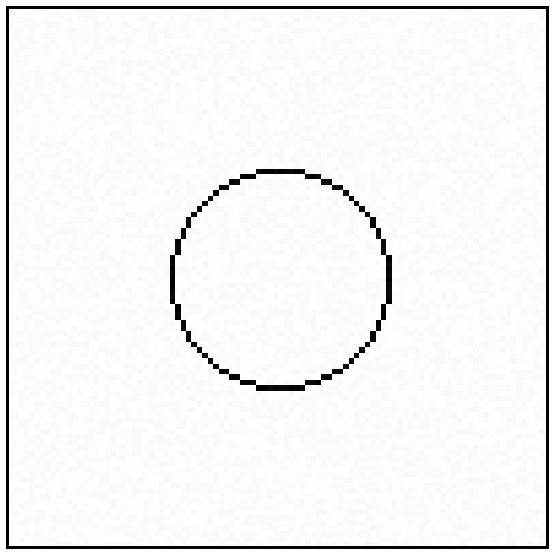
\includegraphics[width=.5in]{../gfx/area.pdf}} & \makecell[tl]{\emph{Area}\\~~~Radius\\~~~+ Position Y \\~~~+ Position X} &~& \makecell[tr]{ ~\\$40$ \\ $800$ \\ $16,000$}\\

	\midrule
	\raisebox{-.85\height}{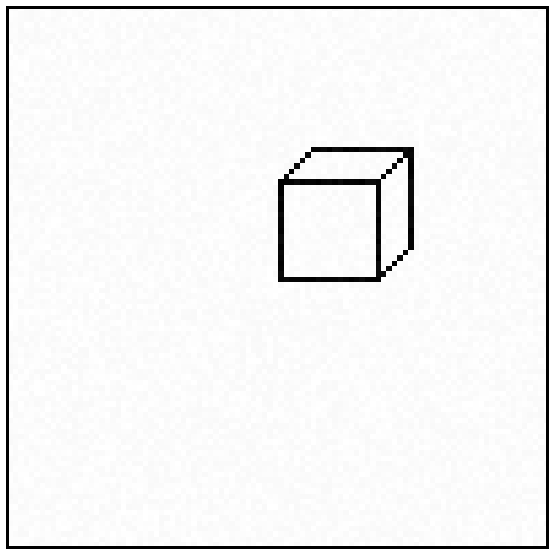
\includegraphics[width=.5in]{../gfx/volume.pdf}} & \makecell[tl]{\emph{Volume}\\~~~Cube Sidelength\\~~~+ Position Y \\~~~+ Position X} &~& \makecell[tr]{ ~\\$20$ \\ $400$ \\ $8,000$}\\
	
	\midrule
	\raisebox{-.85\height}{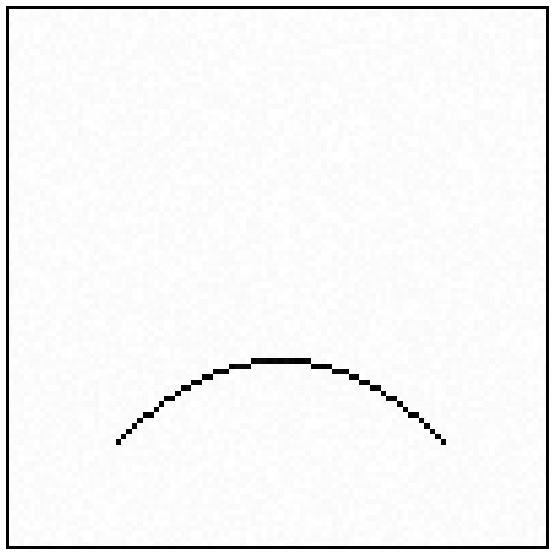
\includegraphics[width=.5in]{../gfx/curvature.pdf}} & \makecell[tl]{\emph{Curvature}\\~~~Midpoint Curvature\\~~~+ Position Y \\~~~+ Position X} &~& \makecell[tr]{ ~\\$80$ \\ $1,600$ \\ $64,000$}\\	

	\midrule
	\raisebox{-.85\height}{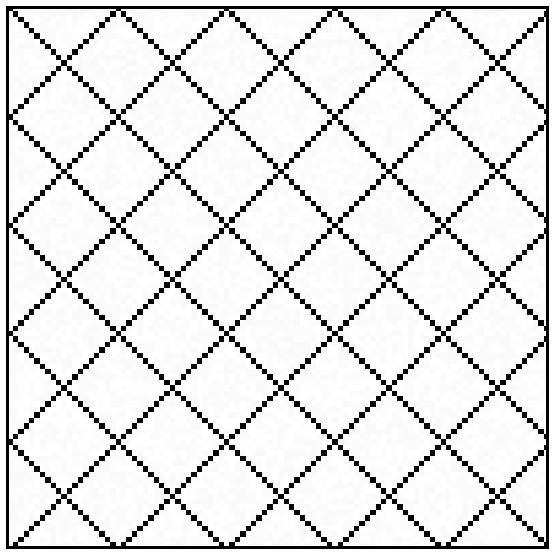
\includegraphics[width=.5in]{../gfx/shading.pdf}} & \makecell[tl]{\emph{Shading}\\~~~Density\\~~~+ Position Y \\~~~+ Position X} &~& \makecell[tr]{ ~\\$100$ \\ $2,000$ \\ $40,000$}\\	
%	
	\bottomrule
\end{tabular}
}
\label{tab:encoding_parameters}
\end{table}


% \subsubsection{Stimuli Generation}
% \JT{Not sure of the value of this.}
% Our code release acts as documentation for our stimuli generation process. Additionally, we describe it below. In all cases, we make sure that the drawn visual marks remain fully on the image, with a border of empty space equal to at least 5$\times$5 so that a first-layer convolution kernel will see all image content.
% \begin{description}
% \item[Position Common Scale] Given a 100$\times$100 image, the task is to estimate a number from 0 to 60. With (0,0) as bottom left, a scale one pixel thick is drawn from (10,20) to (10,80). The position dot is drawn offset from the scale horizontally by 40 pixels, i.e., at (50,.), with variation in Y between 20--80. To add complexity, the horizontal position of the dot then also varies in X (20--80). In the most complex variation, the dot size varies in pixel width/height from the set $\{1, 3, 5, 7, 9, 11\}$, i.e., the dot is maximally 11$\times$11 pixels large.
% \item[Position Non-aligned Scale] This is the same as for `Position Common Scale', with the task being to estimate a number from 0 to 60. Now, the vertical position of the scale now also varied by offsetting by between -10 and 10 pixels, i.e., any 80 pixels within the range 10--90. The dot is similarly offset so that it follows the scale.
% \item[Length] The task is to estimate the bar length, which is randomly generated between 1 and 60. In the simplest case, this is drawn at x-coordinate 50 pixels. Then, we vary the horizontal position between positions 20--80. Finally, we vary the stroke width from the set $\{1, 3, 5, 7, 9, 11\}$.
% \item{Direction}
% \item{Angle}
% \item{Area}
% \item{Volume}
% \item{Curvature}
% \item{Shading}
% \end{description}


\subsection{Position-length Experiment}

\change{
Again, we attempted to replicate Cleveland and McGill's stimuli as closely as possible, while removing the text on the scale and the A/B category labels (Figure~\ref{fig:cmcg_positionlength_comparison}). These values are implicitly encoded by the vertical height within the image, and by the left/right position of the bars. Like Cleveland and McGill, we place a dot within the regions that require ratio estimation. In our case, the network must learn the association of dot placement to required length estimation.
}

\begin{figure*}[tb]
    \centering
    %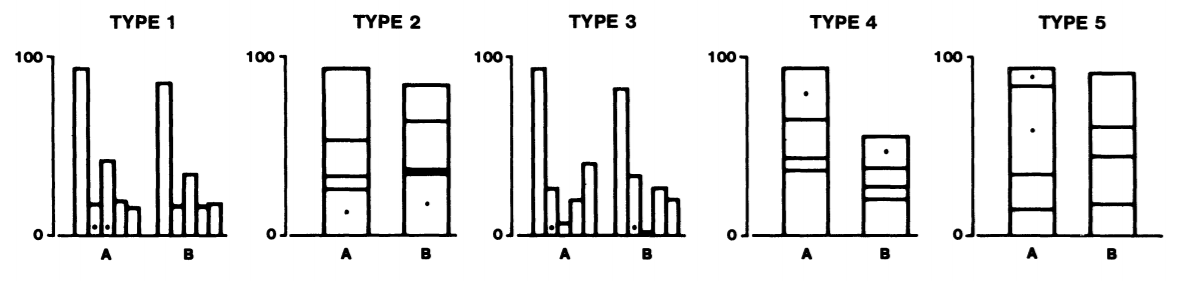
\includegraphics[width=0.8\linewidth]{./gfx/CMcG_Comparison/CMcG_PositionLength.png}\\
    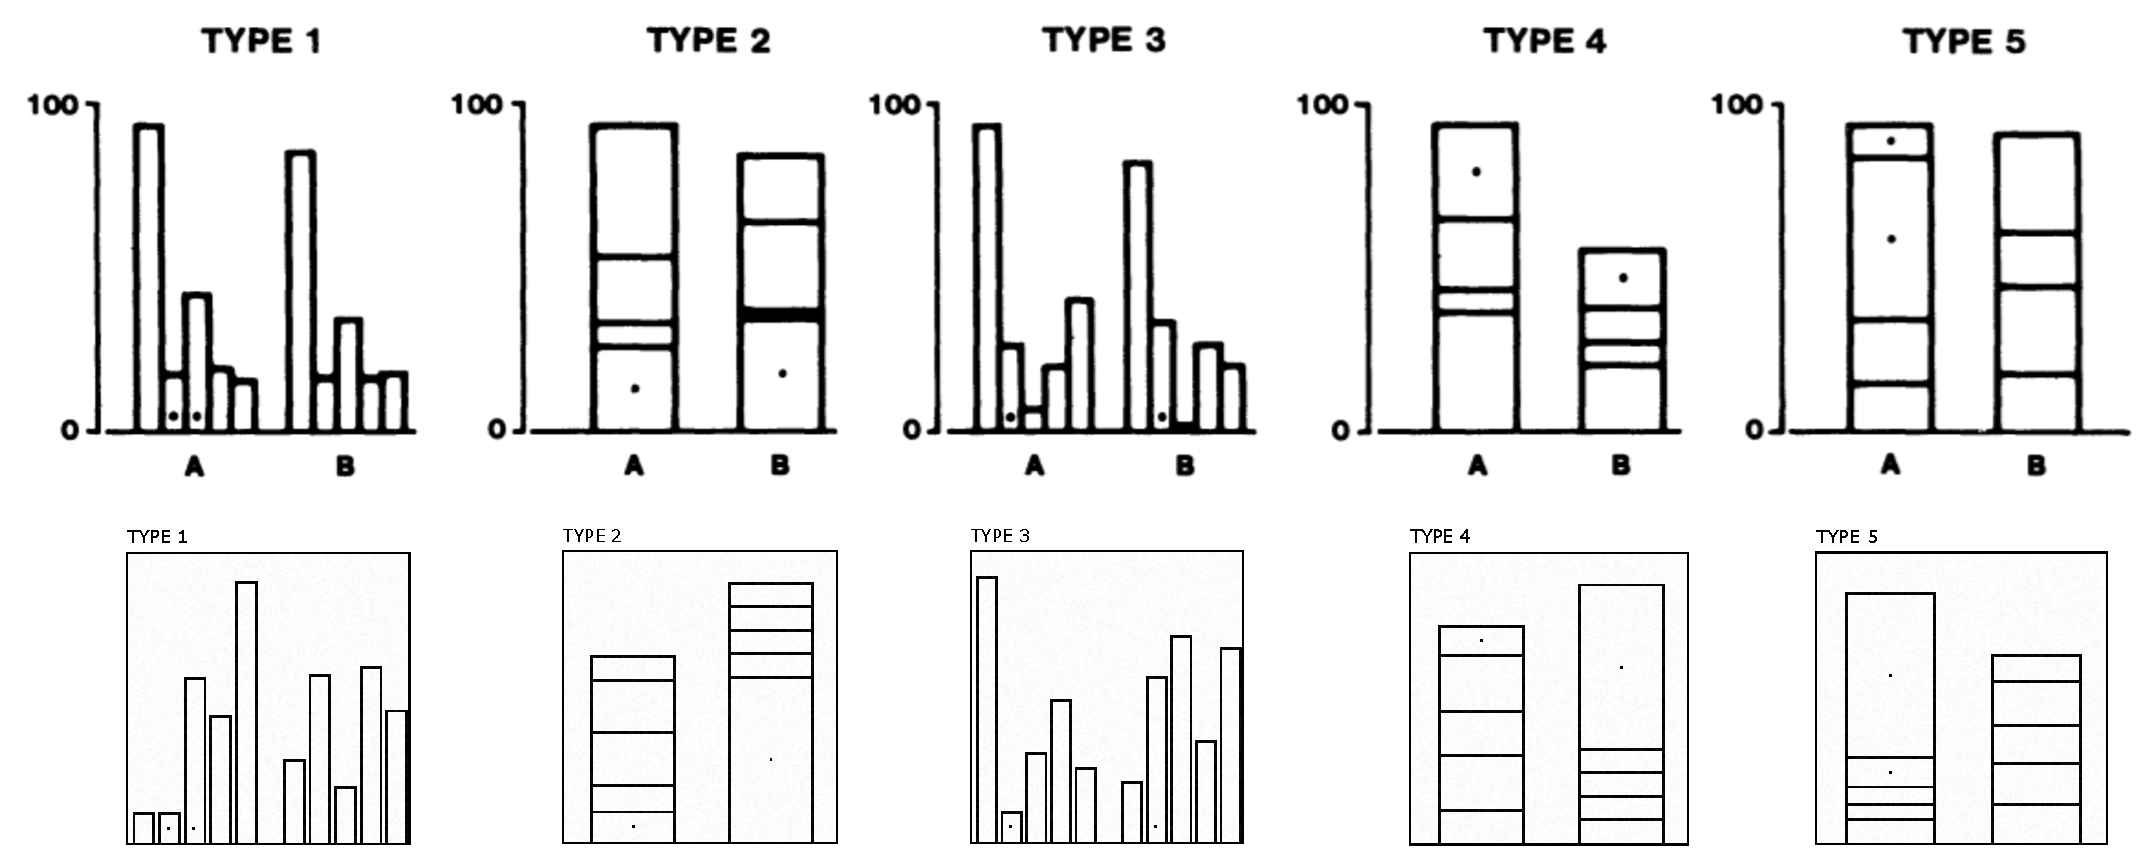
\includegraphics[width=0.8\linewidth]{./gfx/CMcG_Comparison/Ours_PositionLength.pdf}
    \caption{\emph{Top:} Cleveland and McGill's example stimuli for their position-length experiment (Figure 4 from \cite{cleveland_mcgill}). \emph{Bottom:} Example stimuli from our position-length experiment. Note that the border around each of our stimuli only exist in this figure; no border exists in our experiments.}
    \label{fig:cmcg_positionlength_comparison}
\end{figure*}

\subsection{Position-angle Experiment}

\change{
As before, our figures make implicit the scales and labels within these stimuli (Figure~\ref{fig:cmcg_positionangle_comparison}). One difference here is that Cleveland and McGill explicitly tell the participants on a supplemental sheet which pie segment or bar is largest; we replace this signal with a visual dot.
}

\begin{figure}[tb]
    \centering
    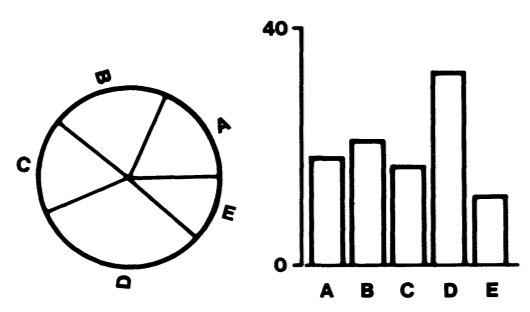
\includegraphics[width=0.75\linewidth,trim=-1cm 0 0 0, clip]{./gfx/CMcG_Comparison/CMcG_PositionAngle.png}\\
    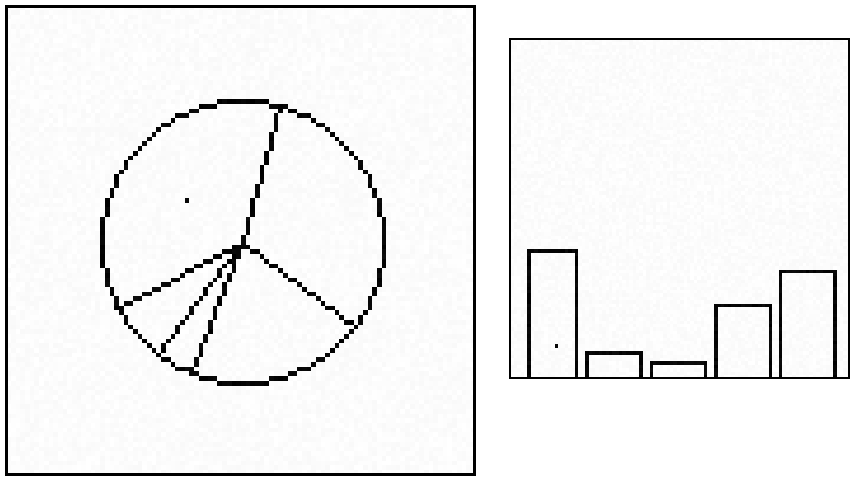
\includegraphics[width=0.72\linewidth]{./gfx/CMcG_Comparison/Ours_PositionAngle.pdf}
    \caption{\emph{Top:} Cleveland and McGill's example stimuli for their position-angle experiment (Figure 3 from \cite{cleveland_mcgill}). \emph{Right:} Example stimuli from our position-length experiment. Note that the border around each of our stimuli only exist in this figure; no border exists in our experiments. Further, we have resized our stimuli on the page to more clearly show the similarity; each are 100$\times$100 pixels.}
    \label{fig:cmcg_positionangle_comparison}
\end{figure}

\subsection{Bars/Rectangles Experiment}

\change{
In this case, the only difference is that we remove the A/B category labels, and let the comparison judgment be implicitly encoded by the left/right bars (Figure~\ref{fig:cmcg_barsrectangles_comparison}).
}

\begin{figure}[tb]
    \centering
    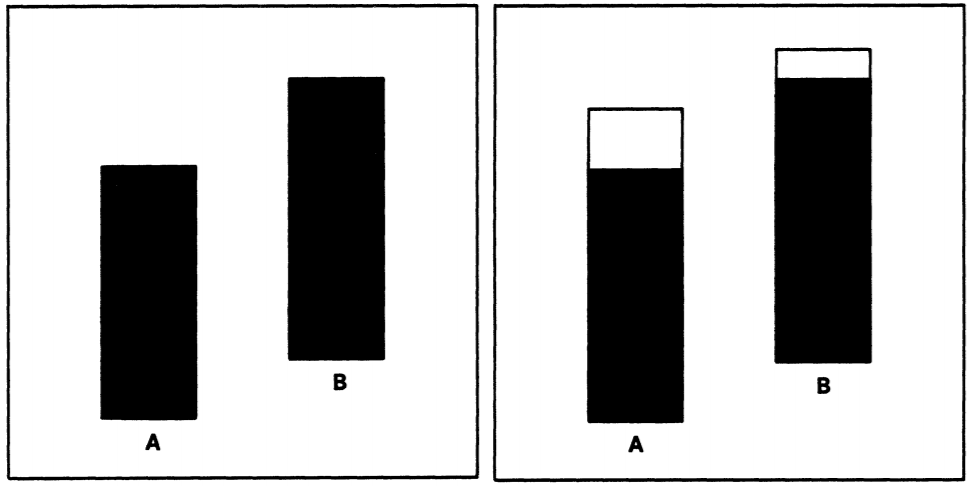
\includegraphics[width=0.8\linewidth]{./gfx/CMcG_Comparison/CMcG_BarsRectangles.png}\\
    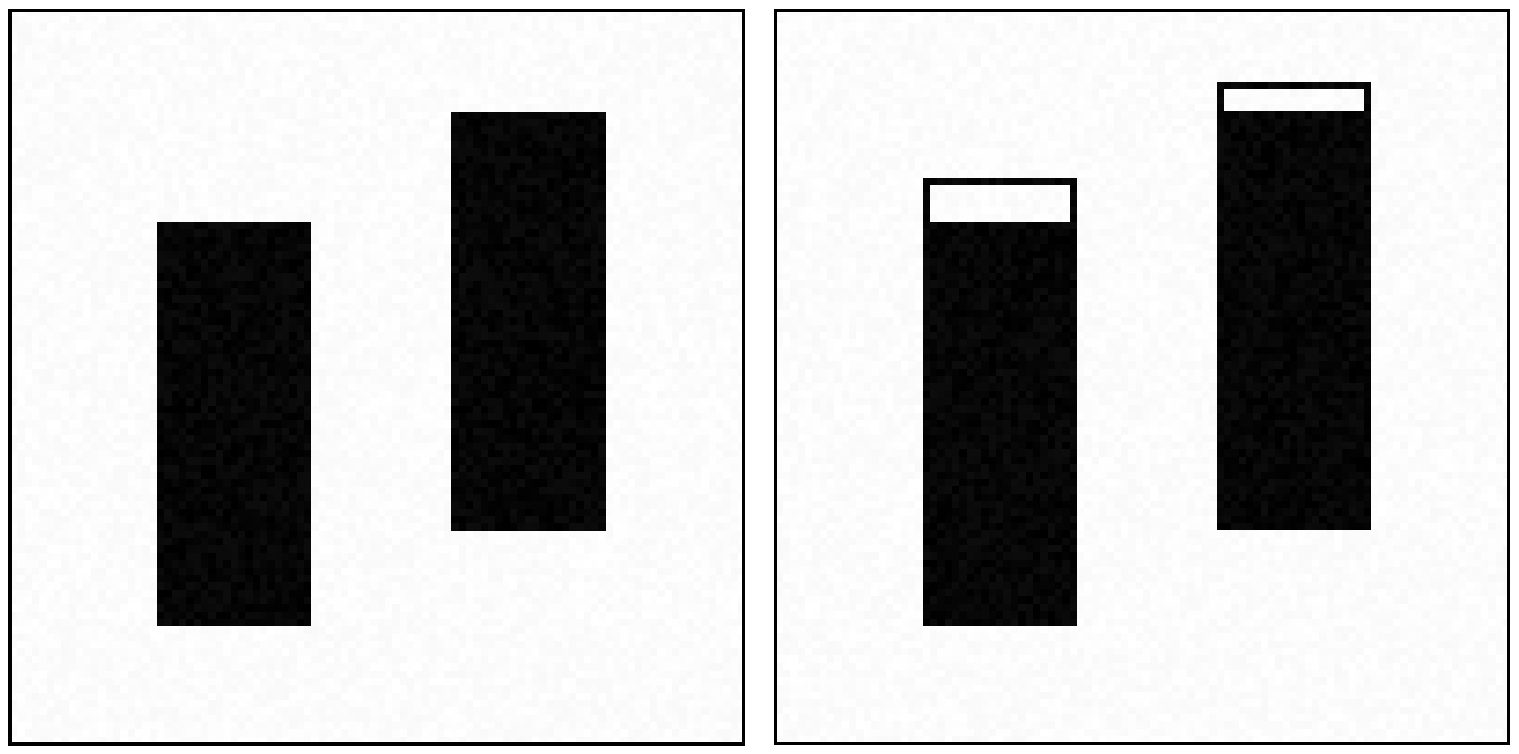
\includegraphics[width=0.8\linewidth]{./gfx/CMcG_Comparison/Ours_BarsRectangles.pdf}
    \caption{\emph{Top:} Cleveland and McGill's example bars and rectangles (Figure 12 from \cite{cleveland_mcgill}). \emph{Right:} Example stimuli from our bars and rectangles experiment. Note that the border around each of our stimuli only exist in this figure; no border exists in our experiments.}
    \label{fig:cmcg_barsrectangles_comparison}
\end{figure}

\subsection{Point Cloud Experiment}

\change{
Cleveland and McGill have no equivalent to this Weber-Fechner's law experiment, and so we show no stimuli comparison.
}


%%%%%%%%%%%%%%%%%%%%%%%%%%%%%%%%%%%%%%%%%%%%%%%%%%%%%%%%%%%%%%%%%%%%%%%%%%%%%%%%%%%%%%%%%%%%%%%%%%%%%%%%%%%%%
\section{\change{Comparing the Human vs.~Machine\\Judgment Processes}}

\change{
There are many general differences in how humans and CNNs perceive: 
\begin{itemize}[itemsep=0.5pt, topsep=1pt, parsep=0.5pt]
    \item Humans have foveal and peripheral vision. 
    \item Humans have explicit attention mechanisms (V1), with neural feedback to drive attention.
    \item Humans have working memory.
    \item Humans can make predictions about what they might see given a hypothesis. 
\end{itemize}    
It can be argued that a CNN can see and integrate all image information at once, as it has no fovea. This partially overcomes the need for attention mechanisms, feedback, and working memory. 

Having spoken to three computational human vision scientists about graphical perception, it is our understanding that we still know very little about how humans see data visualizations beyond the very early visual system. In some cases, through works like Cleveland and McGill, we know how \emph{well} humans can judge elementary graphical perception tasks, and this is the level at which we make comparisons about the suitability of CNNs as models for human graphical perception---implicitly, rather than explicitly.

Given these limitations, we will try and describe at a high level what we think happens when a human is asked to predict from the `position common scale' stimuli, and what happens when a CNN is asked to predict given the stimuli as input.

\subsection{Human Judgment}
For training, a human being learns how to see through experience gained by existing in the world, such as our ability to interpret visual edges as lines and to read numbers. Given this experience, upon observing the `position common scale' stimuli at prediction time:
\begin{enumerate}[label=\arabic*.,itemsep=0.5pt, topsep=1pt, parsep=0.5pt]
    \item The human looks at the scale and reads the demarcation ticks and text labels. This lets the human know the numerical values associated with the visual marks and defines the scale bounds.
    \item The human looks at the dot and mentally projects a horizontal line over to intersect the scale.
    \item The human estimates the distance between the two closest demarcation ticks and the intersection line. The human may make additional mental ticks within the span to help in the estimation.
    \item The human converts this into the scale using knowledge of the tick values, producing a prediction.
\end{enumerate}
The first two steps may be interchanged, as the output of each is stored in human memory in either case.


\subsection{Brief CNN Introduction}
For a CNN, the process is harder to describe in intuitive terms, and so we provide a brief introduction to how CNNs work. The network is defined to have a set of layers, with each layer feeding into the next, and each typically performing some subset of three operations: convolution with kernels, non-linear transformation with activation functions, and pooling. Following these, a densely-connected set of neurons known as a multi-layer perceptron (MLP) learns how to combine the convolution layer outputs to make a prediction.

\paragraph{Trainable Convolution.} The network has a number of kernels within each layer, e.g., in layer one of LeNet, we have 20 trainable 5$\times$5 kernels. We convolve an input image with our kernels to produce a `feature map' measuring the kernel response to the image. Once trained, these kernels identify important visual elements in a scene, similar to a template matching process. In a loose biological comparison, kernels in early layers are often compared to functions in the early human visual system that identify contrast or edges, which is an important task within graphical perception. Through hierarchical combination, kernels in later layers are said to localize and identify objects (if the network is trained on natural images)~\cite{Zeiler2014}. In our graphical perception setting, this would potentially let a network identify and compare larger structures like the cube in our volume task, or glyphs.

\paragraph{Activation Functions.} With the feature maps computed by the convolution with trained kernels, we apply the activation function, which defines how much we wish our network to respond to a given feature. LeNet uses the Rectified Linear Unit (ReLU) activation function, which sets all values less than 0 to 0, and is loosely said to be biologically inspired by one-sided human neuron activations. ReLU helps us train deeper neural networks by propagating large positive signals~\cite{pmlr-v15-glorot11a}.

\paragraph{Pooling.} A pooling layer acts to summarize a response over a spatial region of the feature map, either by averaging or by selecting the highest response from the region (`max.~pooling'). LeNet uses 2$\times$2 max pooling, which decreases the size of the feature map by two in each dimension. Across layers, pooling lets the network accumulate or select activations as part of its prediction process.

\paragraph{MLP.} Finally, after a series of layers (two for LeNet: Conv$\rightarrow$ReLU$\rightarrow$MaxPool$\rightarrow$Conv$\rightarrow$ReLU$\rightarrow$MaxPool), we feed the resulting downsampled feature map into a multi-layer perceptron, which is connected to every pixel in the feature map. Each perceptron in the MLP is a linear classifier that is trained to weight the feature maps to produce the correct prediction. The MLP itself has two layers separated by a ReLU to allow for complex combination.

\subsection{CNN Judgment.} Now, let us predict for the `position common scale' task. Through training, our network has learned a set of convolutional kernels across its layers that, in combination, help the network to predict estimates for unseen test data.
\begin{enumerate}[label=\arabic*.,itemsep=0.5pt, topsep=1pt, parsep=0.5pt]
    \item The kernels produce strong responses in parts of the test image that were helpful to predict the training data. These are typically edges or visualization parts such as bars. For `position common scale', early-layer kernels produce a strong response for dots.
    \item Pooling selects the most important features from across the image. Over a hierarchy of layers, these are trained to be combined by kernels into more useful features. For `position common scale', this dot response would be propagated through the layers, but the exact position of the dot would be made imprecise.
    \item The MLP has been trained to weight (or combine) the pooled feature maps into a prediction. For `position common scale', the MLP will weight the feature map response at different locations to map to a value between 0--60.
\end{enumerate}

\subsection{Human/CNN Comparison}
While parts of this process are similar, such as the early visual system identifying edges, the high-level picture is that the human and CNN prediction processes are substantially different. The human prediction involves implicit geometric understanding of a space, with projection and line length comparisons. The CNN prediction has no explicit way to represent these high-level operations; instead, they must be implicitly represented though a series of low-level weighted sums of pixel responses, clamping activation function transformations, and spatially-local max operations. 

However, for some perception tasks like area estimation or our point cloud experiment in the main paper, this series of operations is beneficial. For instance, estimating the number of points added to the point cloud can be computed exactly by summing over the stimuli and subtracting the base number of points (10, 100, 1,000). This is a task that is extremely tedious at best for a human, but easier for the CNN given its layer aggregation methodology.
%Given the training data, the CNN is able to interpolate its trained response to new examples of sufficient similarity. But, as we show in the main paper, this generalization is limited for many of our tasks. 
}

%%%%%%%%%%%%%%%%%%%%%%%%%%%%%%%%%%%%%%%%%%%%%%%%%%%%%%%%%%%%%%%%%%%%%%%%%%%%%%%%%%%%%%%%%%%%%%%%%%%%%%%%%%%%%
\section{Supplemental Results}

We present several plots that contain complete results for the elementary perceptual task experiment, for which, given the number of experiments, the main paper presented only a selection. We report MLAE for all added parameters to the stimuli, rather than just the most complex parameterization as in the main paper (Figures~\ref{fig:epc_mlae} and \ref{fig:epc_mlae_boxplots}). From this, we see that performance is largely equal across parameters, showing that most networks have sufficient capacity for the given parameterizations.

We also report complete results for the cross-network variability experiment on the elementary perceptual task experiment (Figure \ref{fig:cross_network}). As in the main paper, this shows that our networks are not able to generalize to additional translation or stroke width parameters without representative training data.

Further, we show how the errors for each network are distributed, across elementary perceptual tasks and across different cross-validation splits (Figure~\ref{fig:errors}). Most errors are approximately normally distributed, though our CNN with less parameters (LeNet) and our MLP often have errors that are farther from a normal distribution and show structure.


%%%%%%%%%%%%%%%%%%%%%%%%%%%%%%%%%%%%%%%%%%%%%%%%%%%%%%%%%%%%%%%%%%%%%%%%%%%%%%%%%%%%%%%%%%%%%%%%%%
%\bibliographystyle{abbrv}
\bibliographystyle{abbrv-doi}
%\bibliographystyle{abbrv-doi-narrow}
%\bibliographystyle{abbrv-doi-hyperref}
%\bibliographystyle{abbrv-doi-hyperref-narrow}

\bibliography{paper}
%%%%%%%%%%%%%%%%%%%%%%%%%%%%%%%%%%%%%%%%%%%%%%%%%%%%%%%%%%%%%%%%%%%%%%%%%%%%%%%%%%%%%%%%%%%%%%%%%%


\begin{figure*}[tbhp]
	\centering
		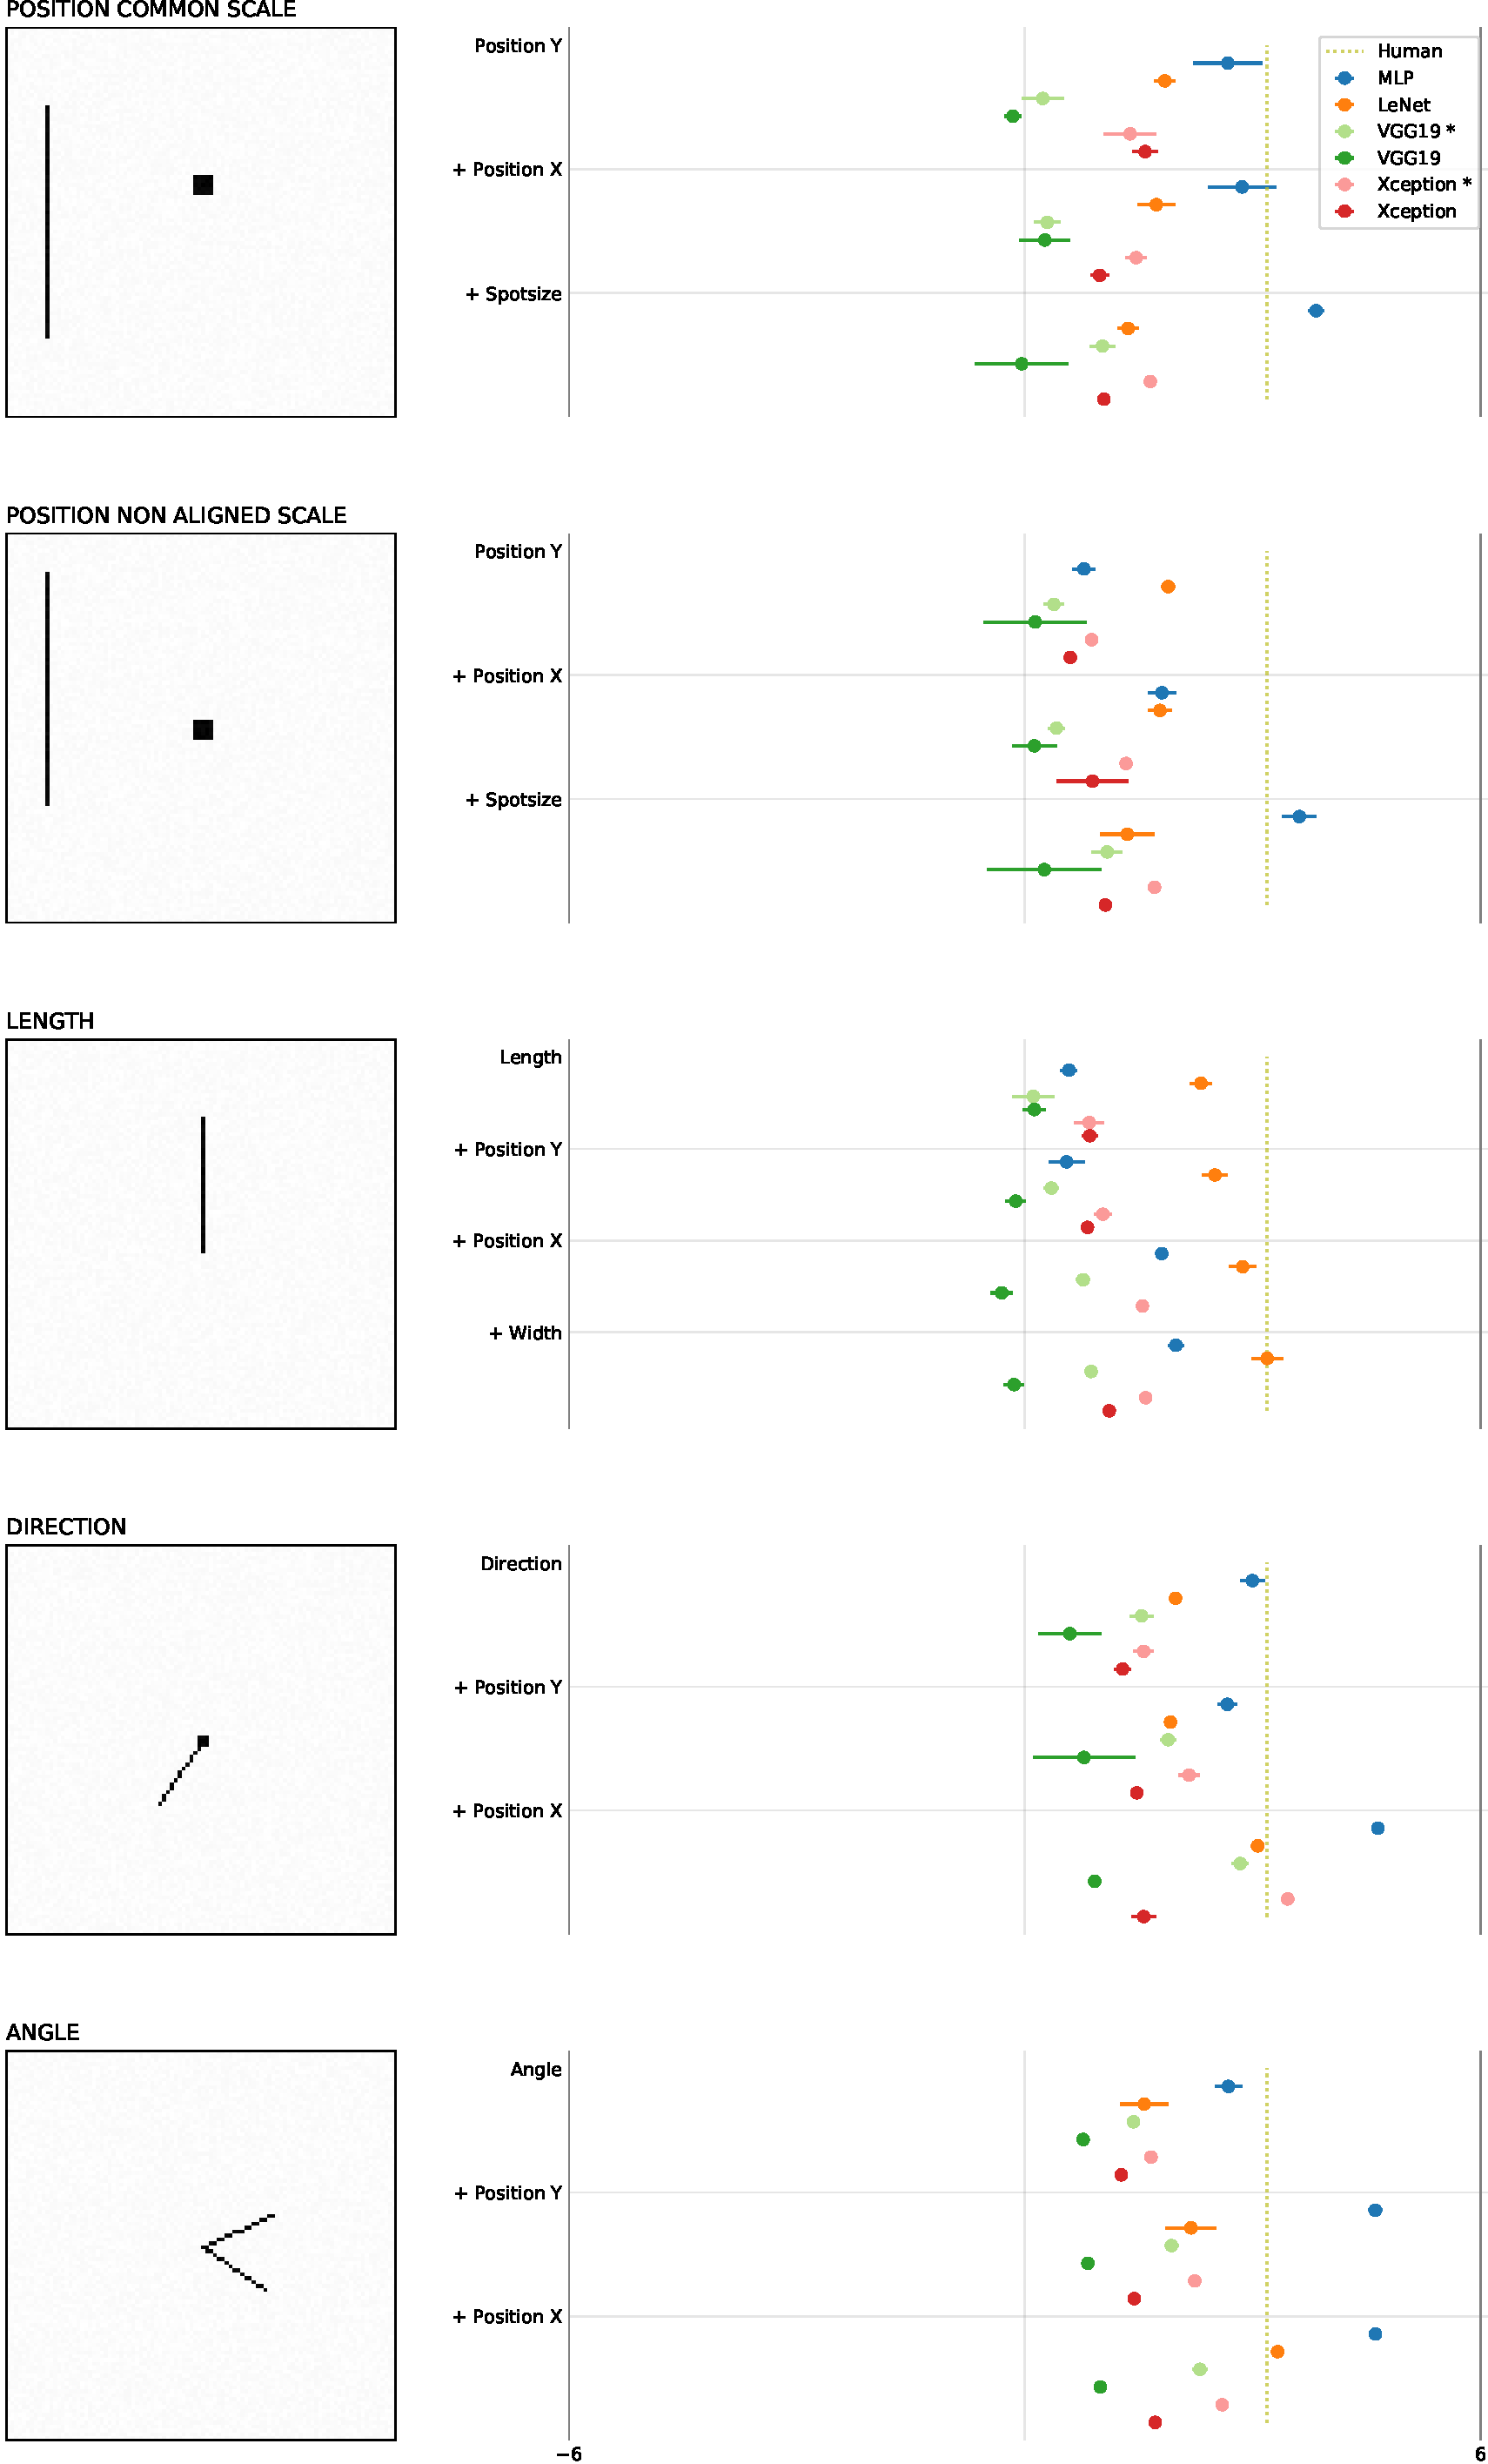
\includegraphics[width=.48\linewidth]{../gfx/figure1_slim_left.pdf}
	  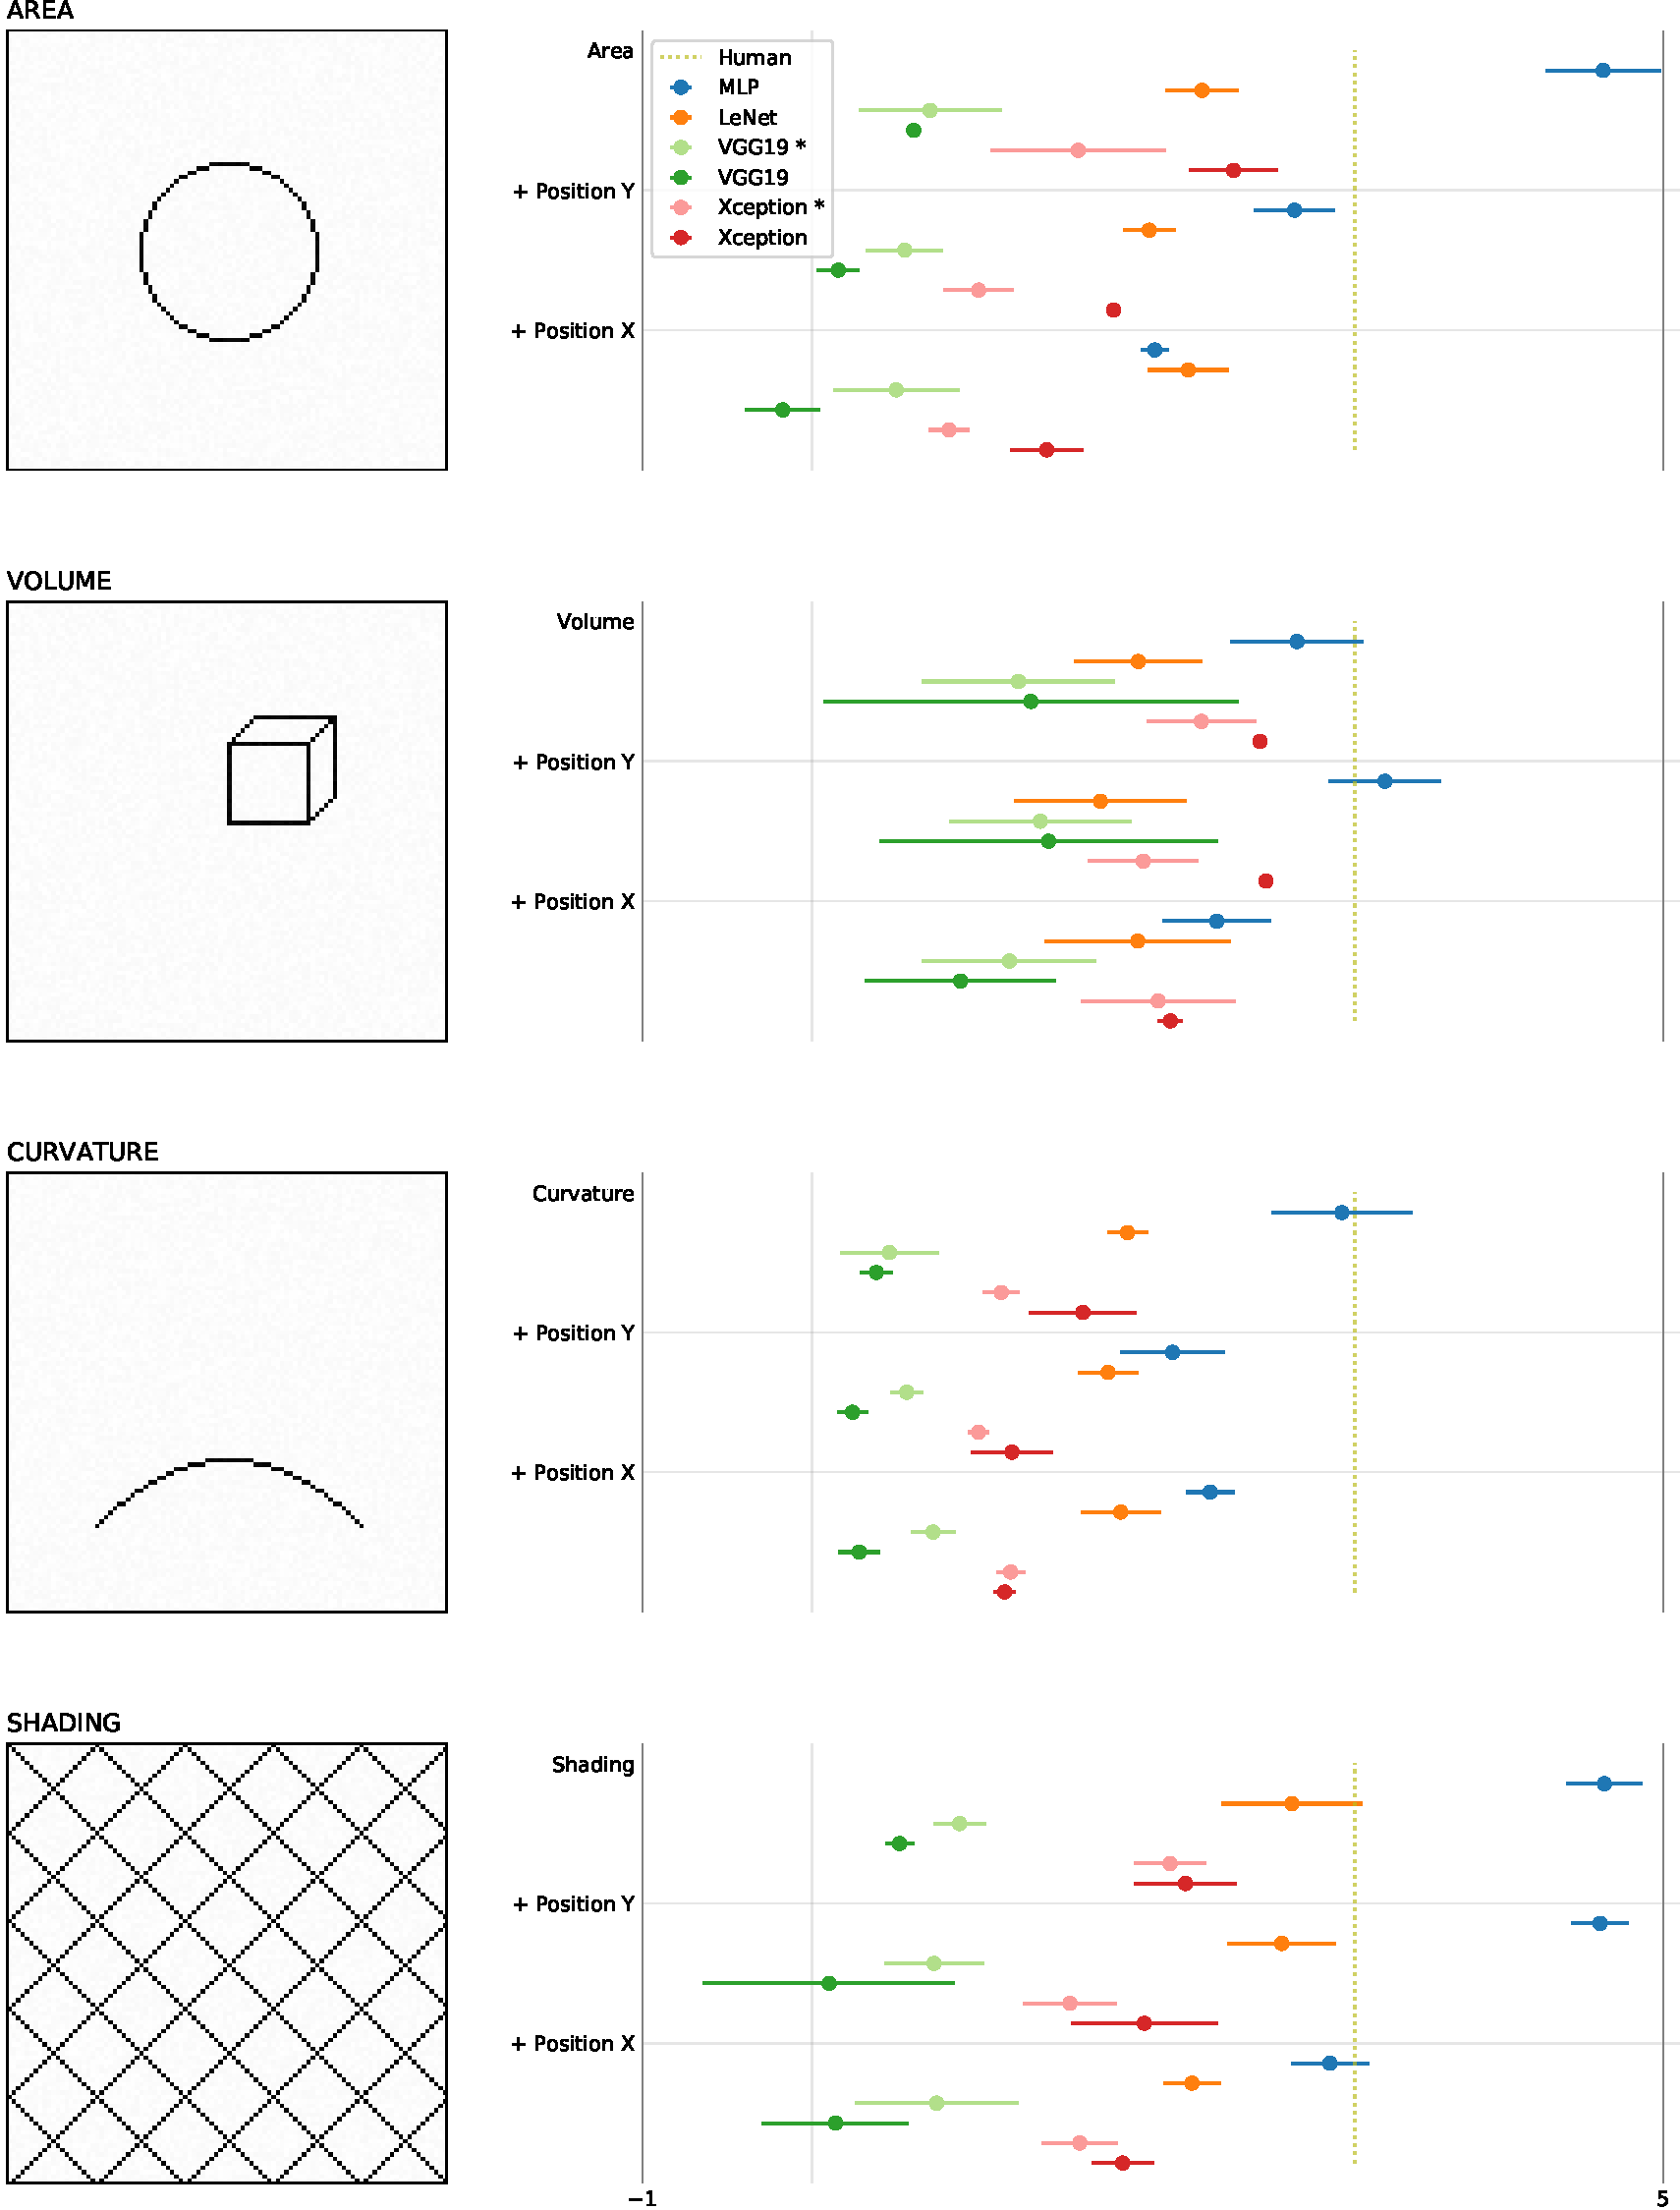
\includegraphics[width=.48\linewidth]{../gfx/figure1_slim_right.pdf}
  \caption{\textbf{Elementary perceptual tasks.} Midmean logistic absolute errors (MLAE) for all generated stimuli and across all networks. The * indicates networks that use ImageNet weights instead of being trained from scratch.}
	\label{fig:epc_mlae}
\end{figure*}

\begin{figure*}[tbhp]
	\centering
		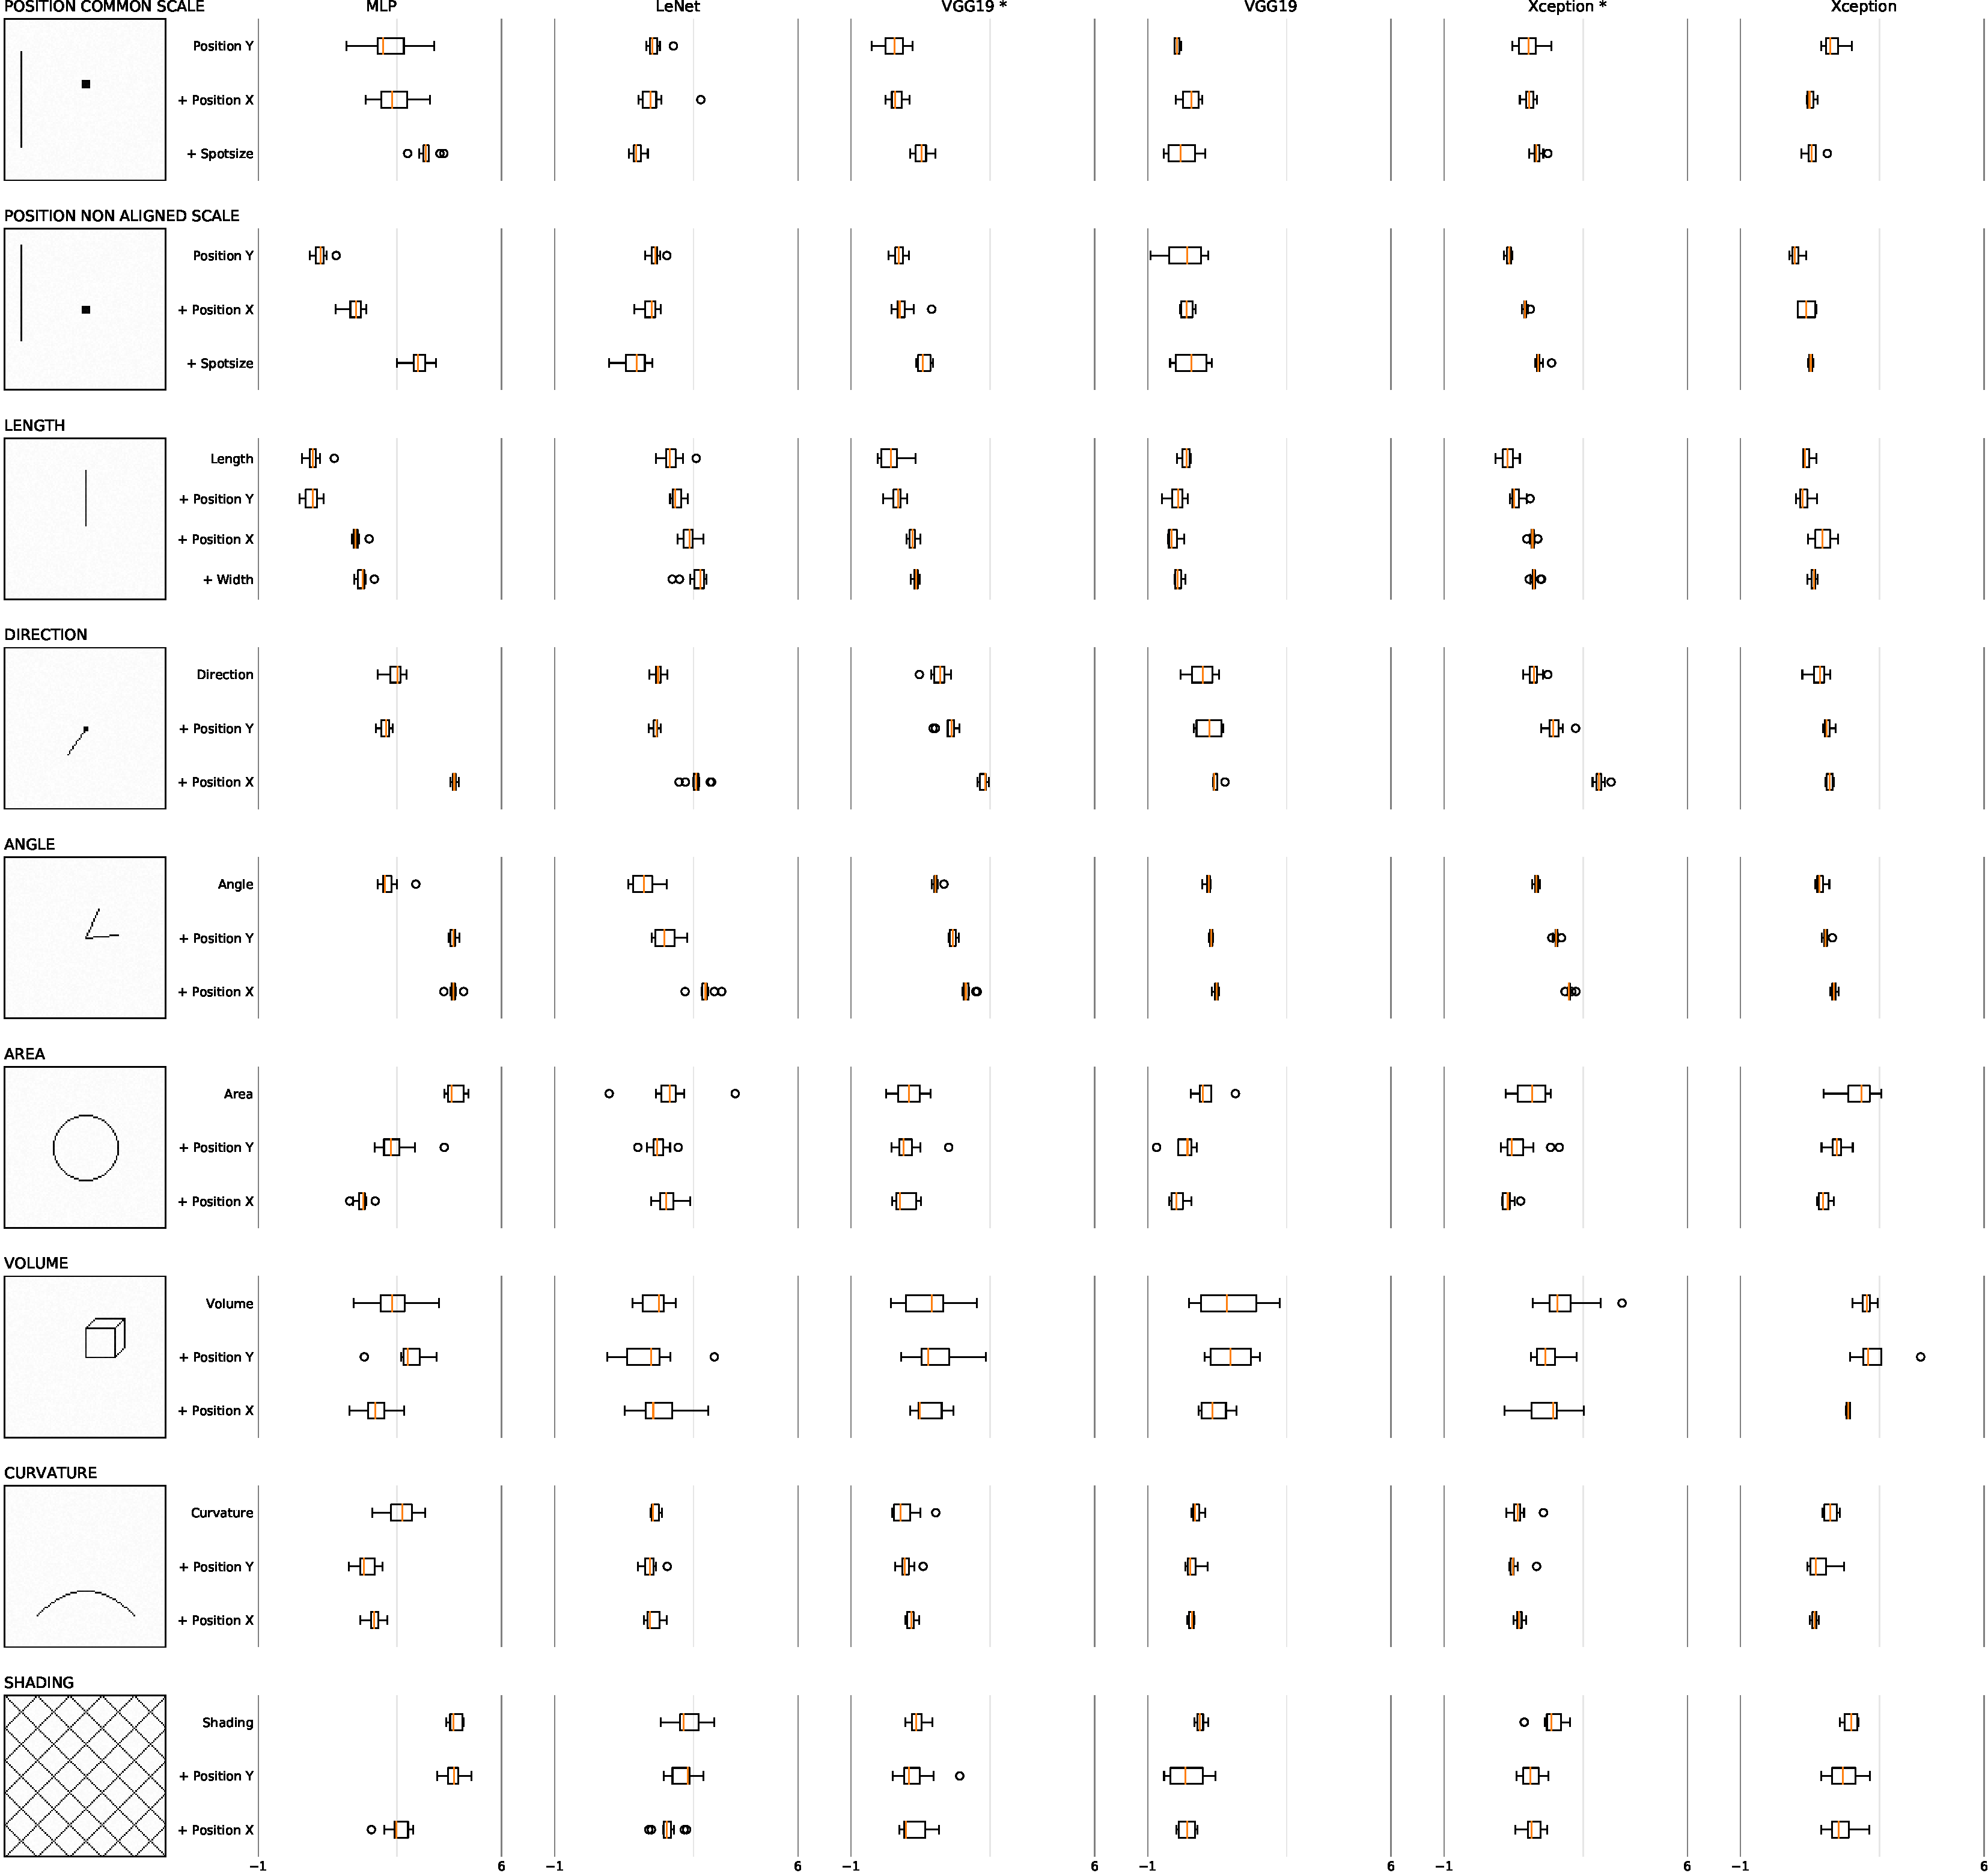
\includegraphics[width=\linewidth]{../gfx/figure1_boxplot_new.pdf}
  \caption{\textbf{Elementary perceptual tasks.} Midmean logistic absolute errors (MLAE) visualized as box plots.}
	\label{fig:epc_mlae_boxplots}
\end{figure*}

\begin{figure*}[tbhp]
	\centering
	  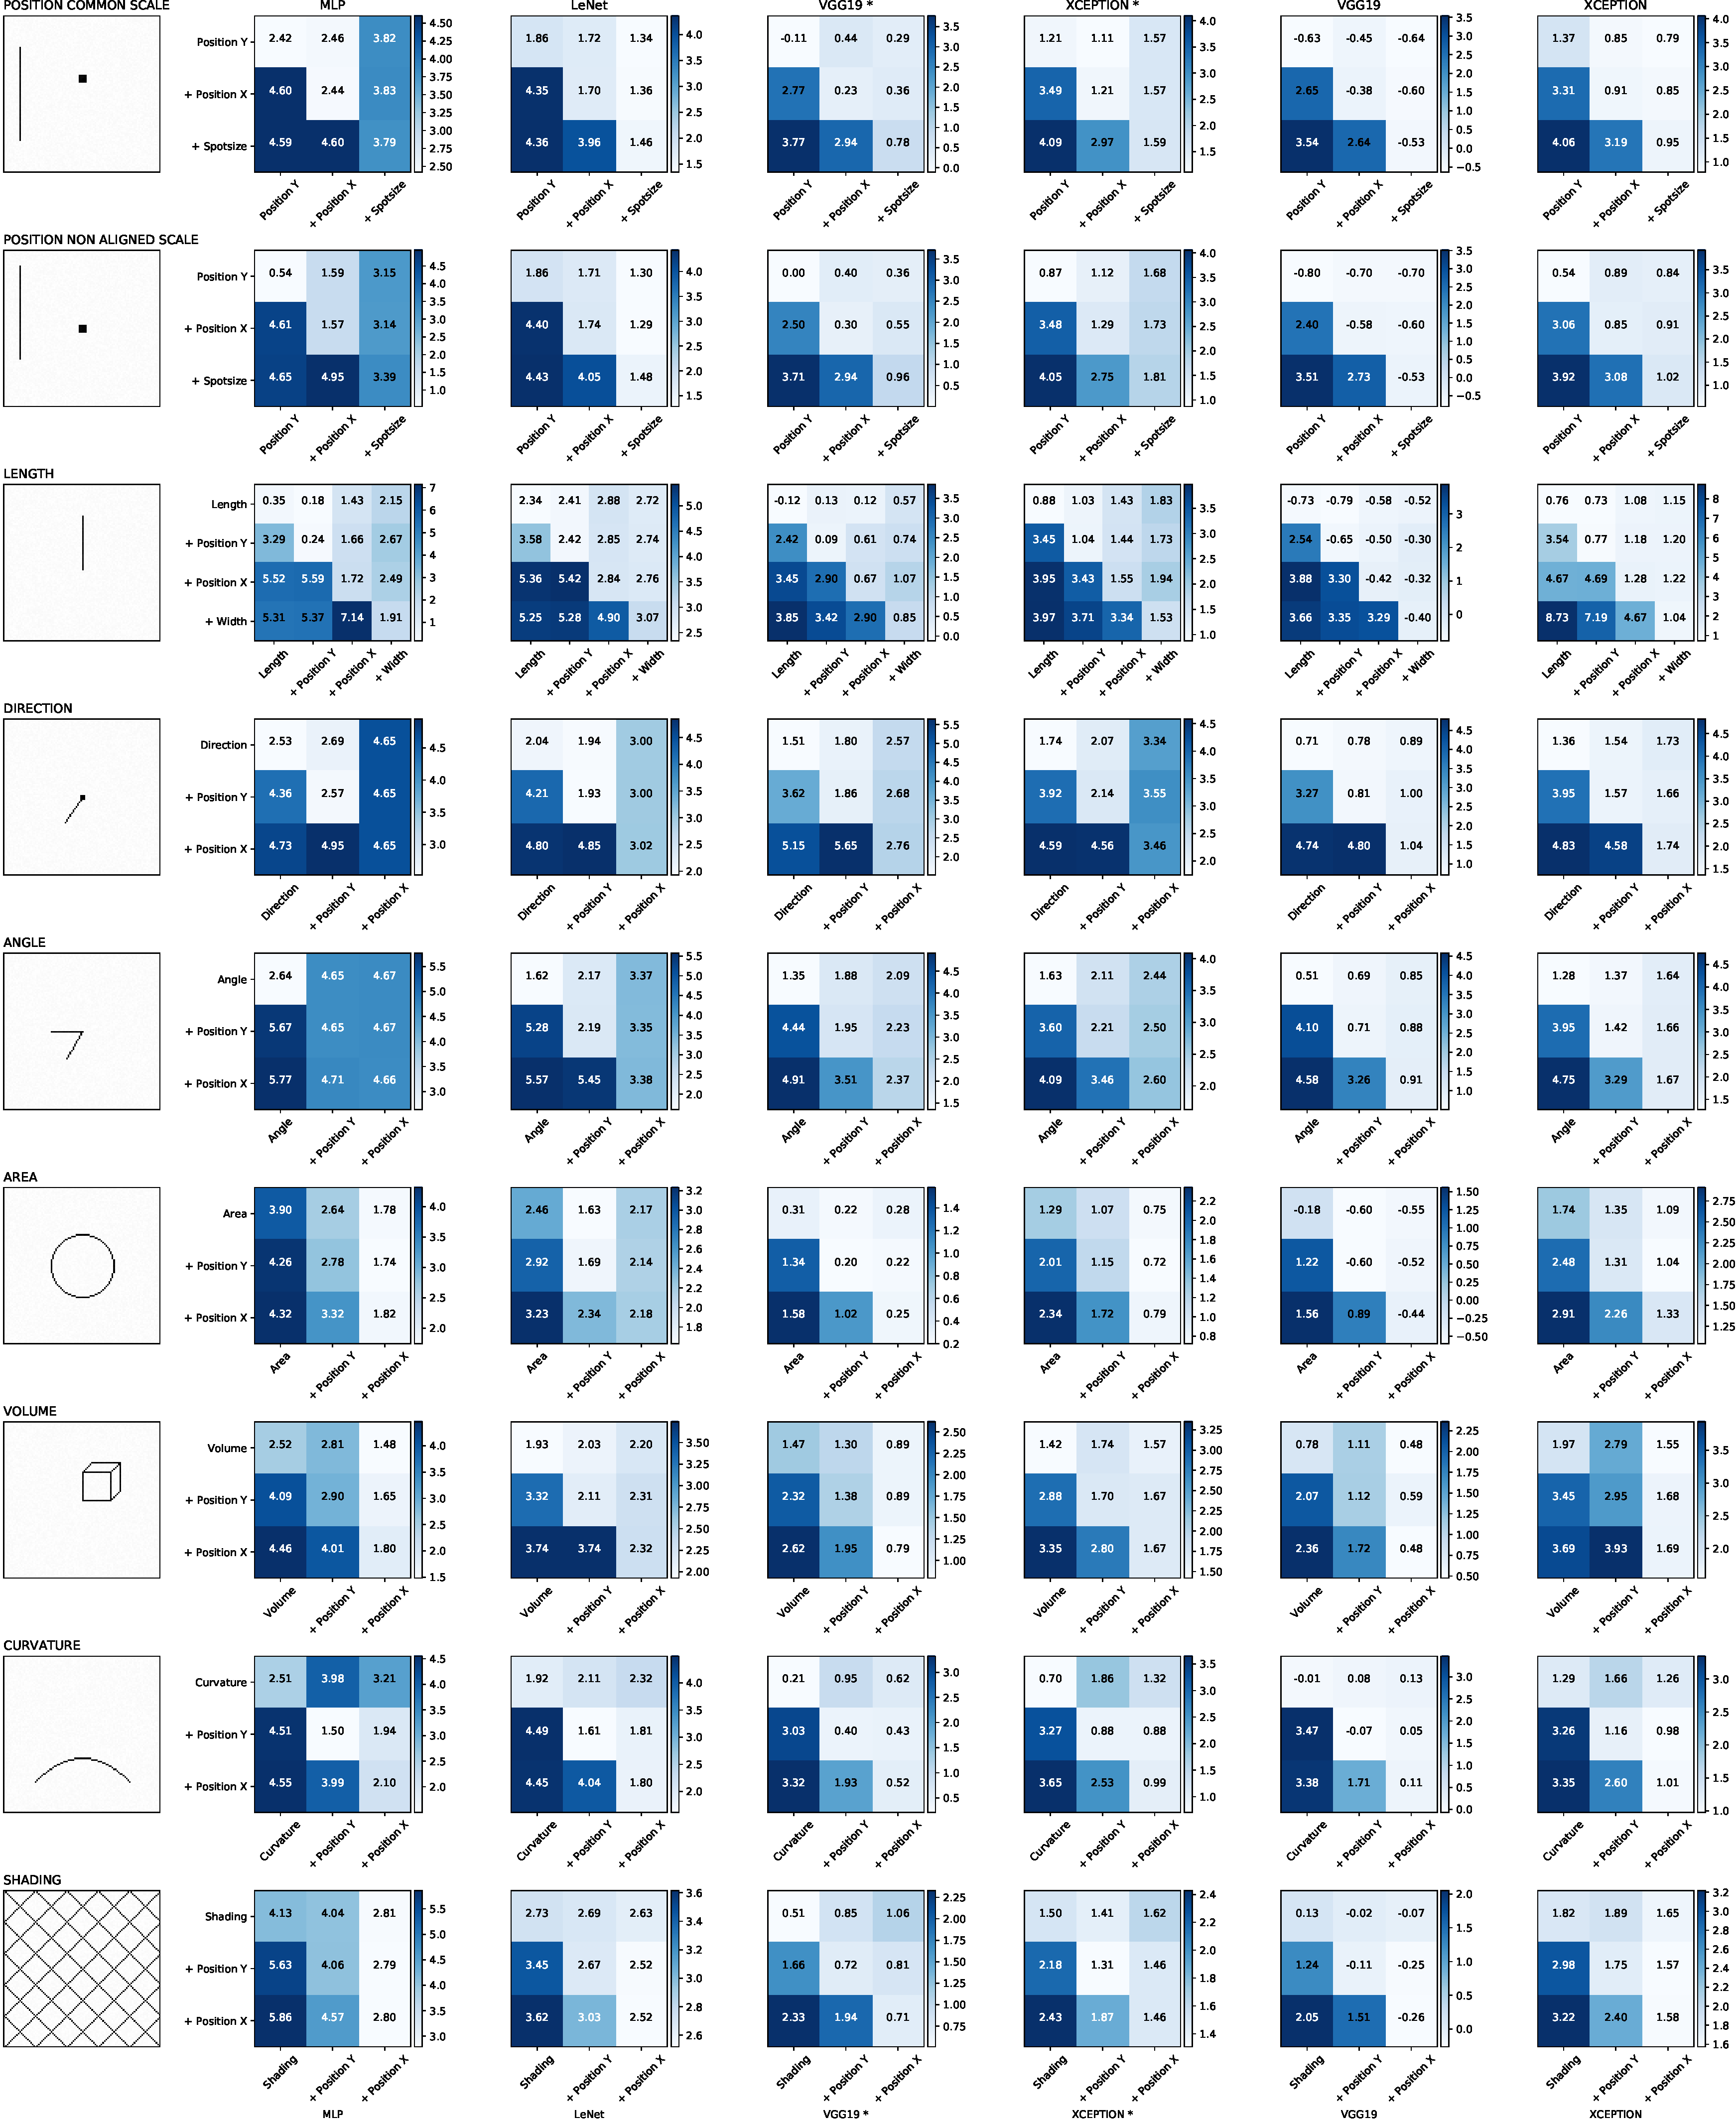
\includegraphics[width=\linewidth]{cross_network_new.pdf}
  \caption{\textbf{Cross-network variability.} Our networks fail when the stimuli changes through translation or stroke width. The x-labels indicate the training configuration while the y-labels indicate the stimuli variation. Numbers represent MLAE.}
	\label{fig:cross_network}
\end{figure*}

\begin{figure*}[tbhp]
	\centering
	  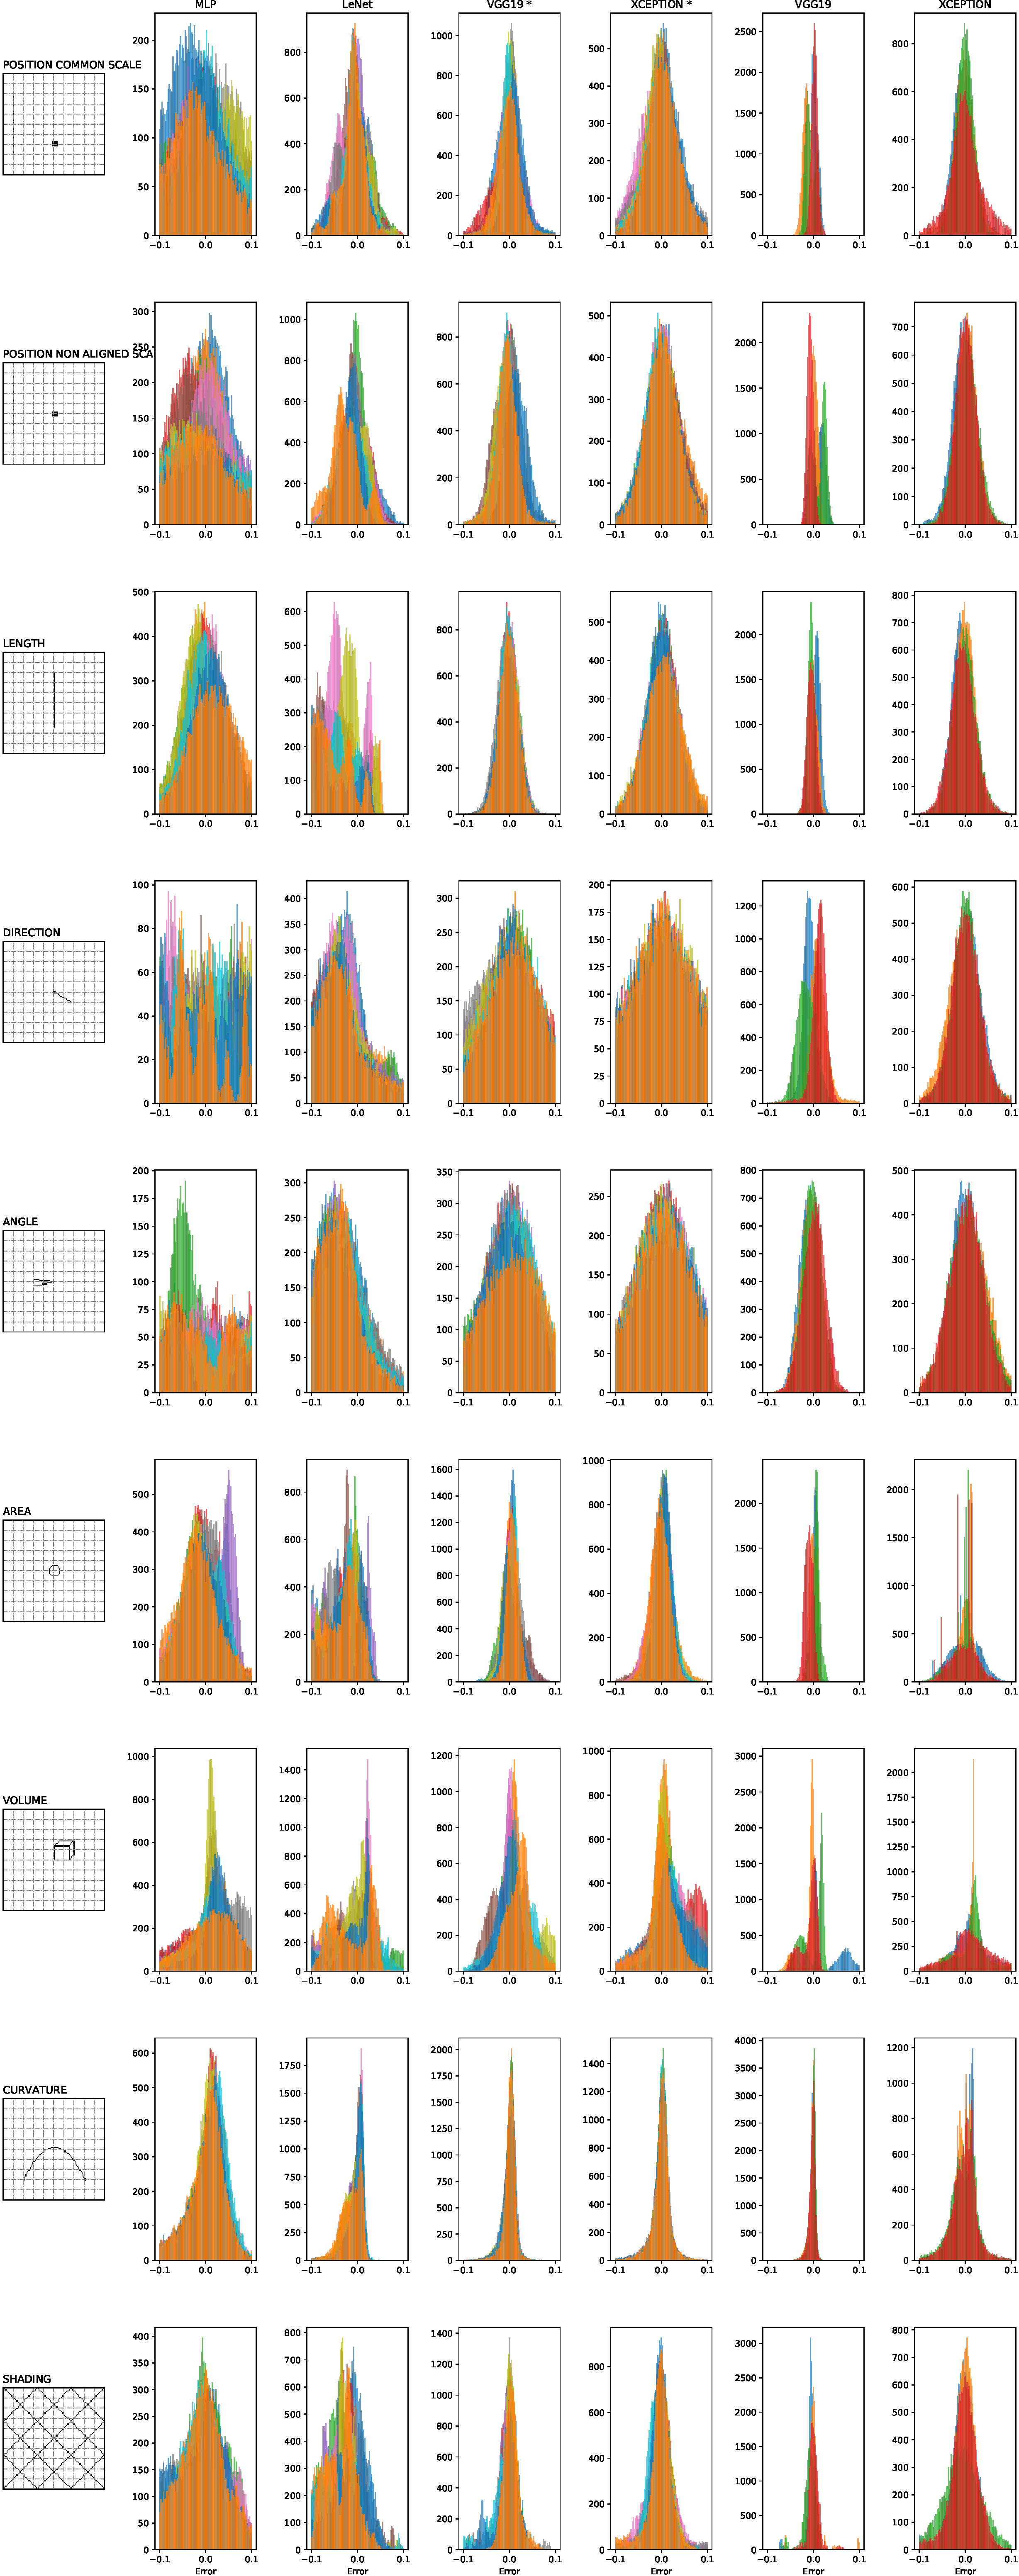
\includegraphics[width=.8\linewidth]{error_inspection_new.pdf}
  \caption{\textbf{Error distributions.} Error distributions of our networks when decoding elementary perceptual tasks.}
	\label{fig:errors}
\end{figure*}

\begin{figure}[tbhp]
	\centering
	  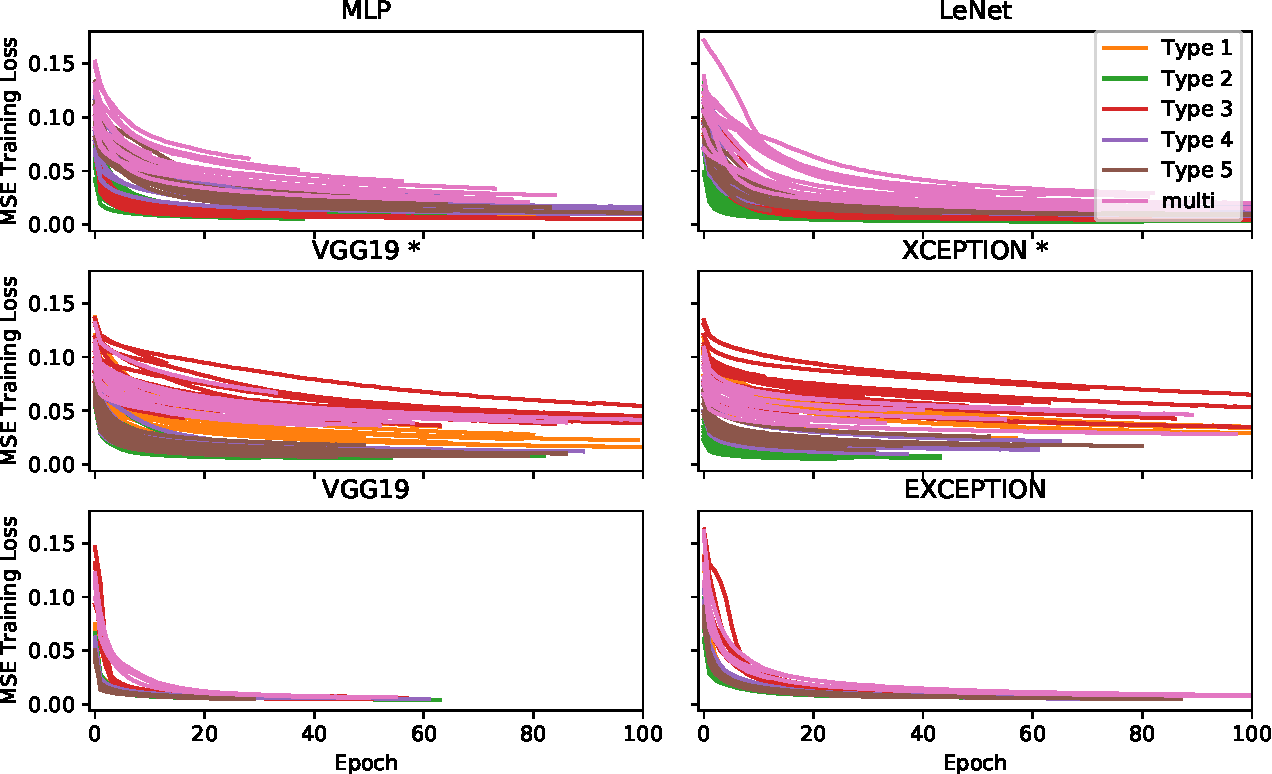
\includegraphics[width=\linewidth]{../gfx/figure4_training_loss_with_multi.pdf}
	  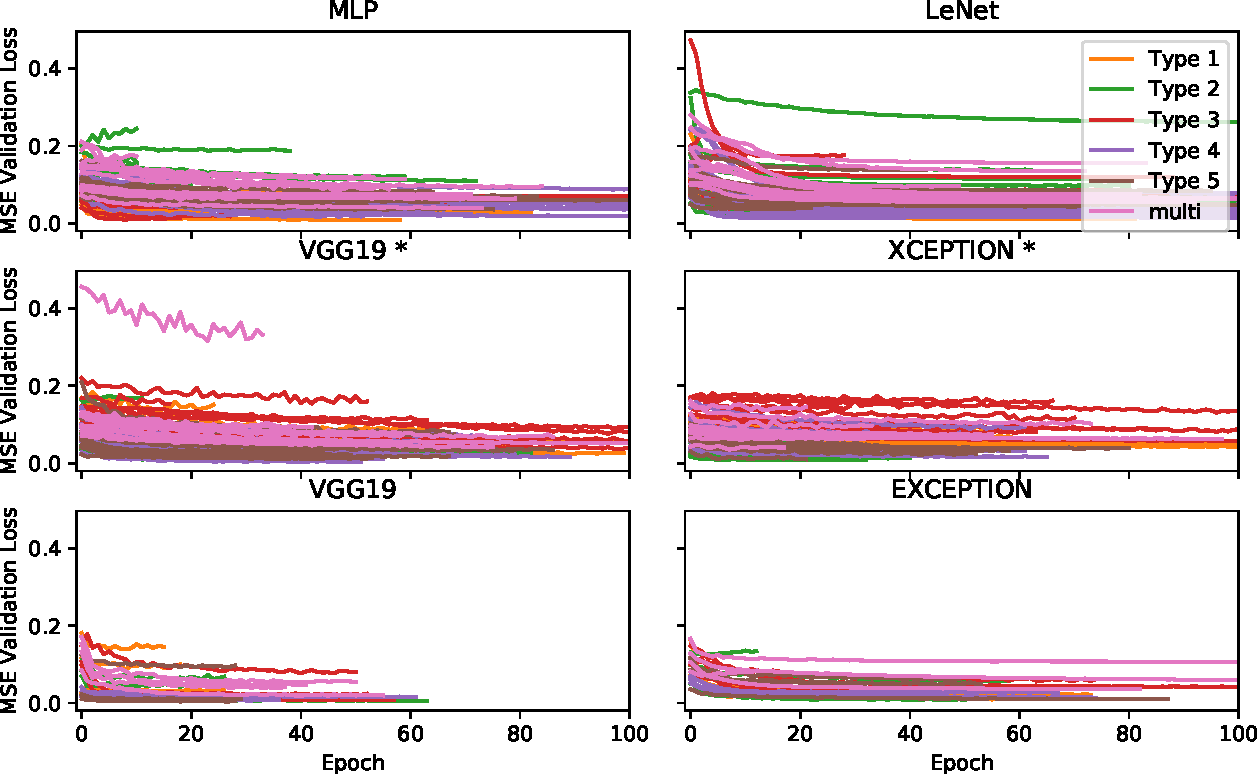
\includegraphics[width=\linewidth]{../gfx/figure4_val_loss_with_multi.pdf}
  \caption{\textbf{Loss plots for the position-length experiment.} We visualize the MSE loss on training data and for unseen validation data after each epoch. There is no significant difference in convergence for either encoding.}
	\label{fig:fig4_loss}
\end{figure}

\begin{figure}[tbhp]
	\centering
	  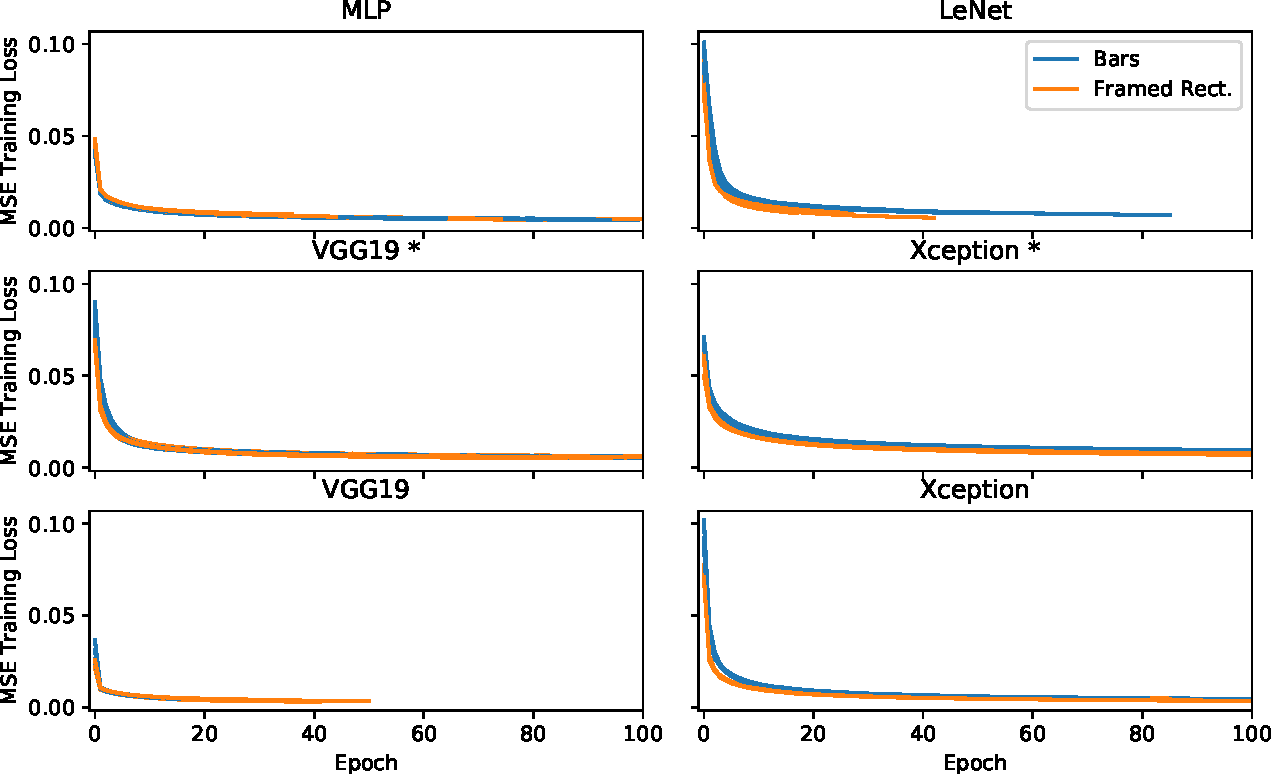
\includegraphics[width=\linewidth]{../gfx/figure12_training_loss.pdf}
	  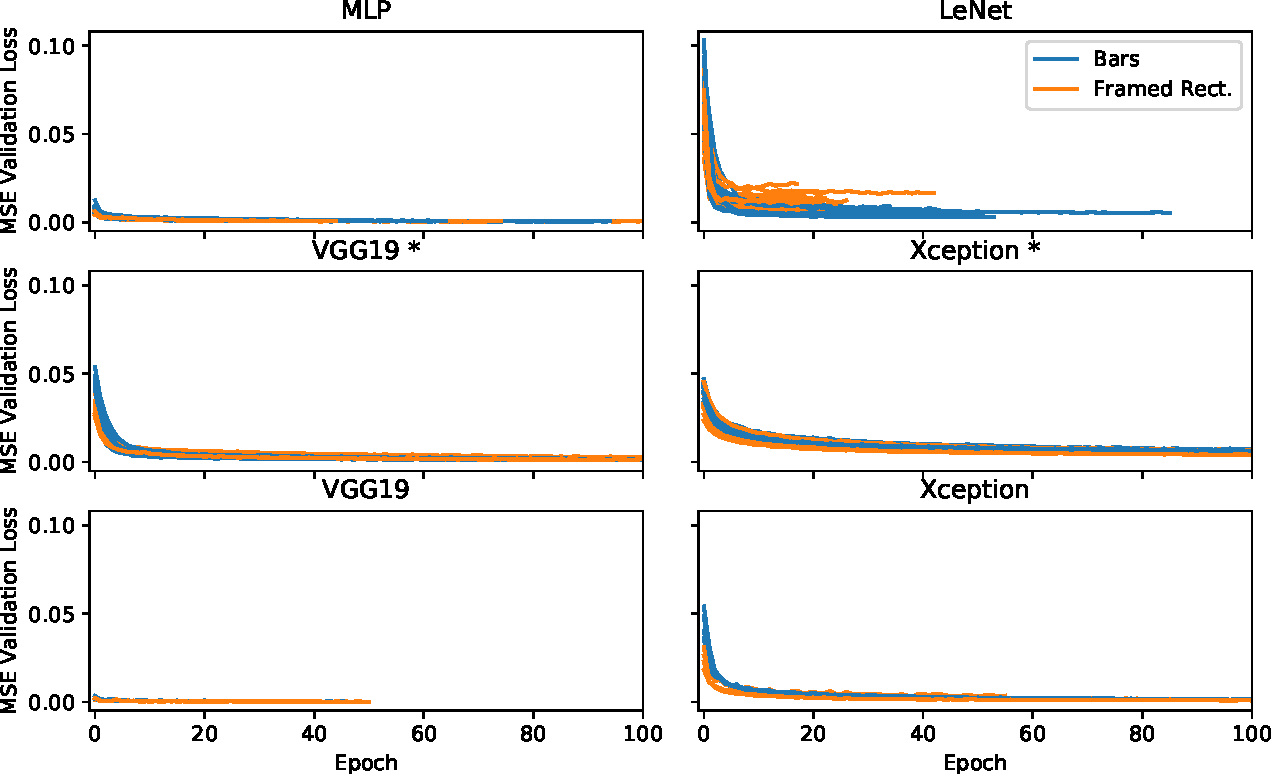
\includegraphics[width=\linewidth]{../gfx/figure12_val_loss.pdf}
  \caption{\textbf{Loss plots for the bars-and-framed-rectangles experiment.} We visualize the MSE loss on training data and for unseen validation data after each epoch. There is no significant difference in convergence for either encoding.}
	\label{fig:fig12_loss}
\end{figure}

\begin{figure*}[tbhp]
	\centering
	
    \subfloat[without noise]{
	  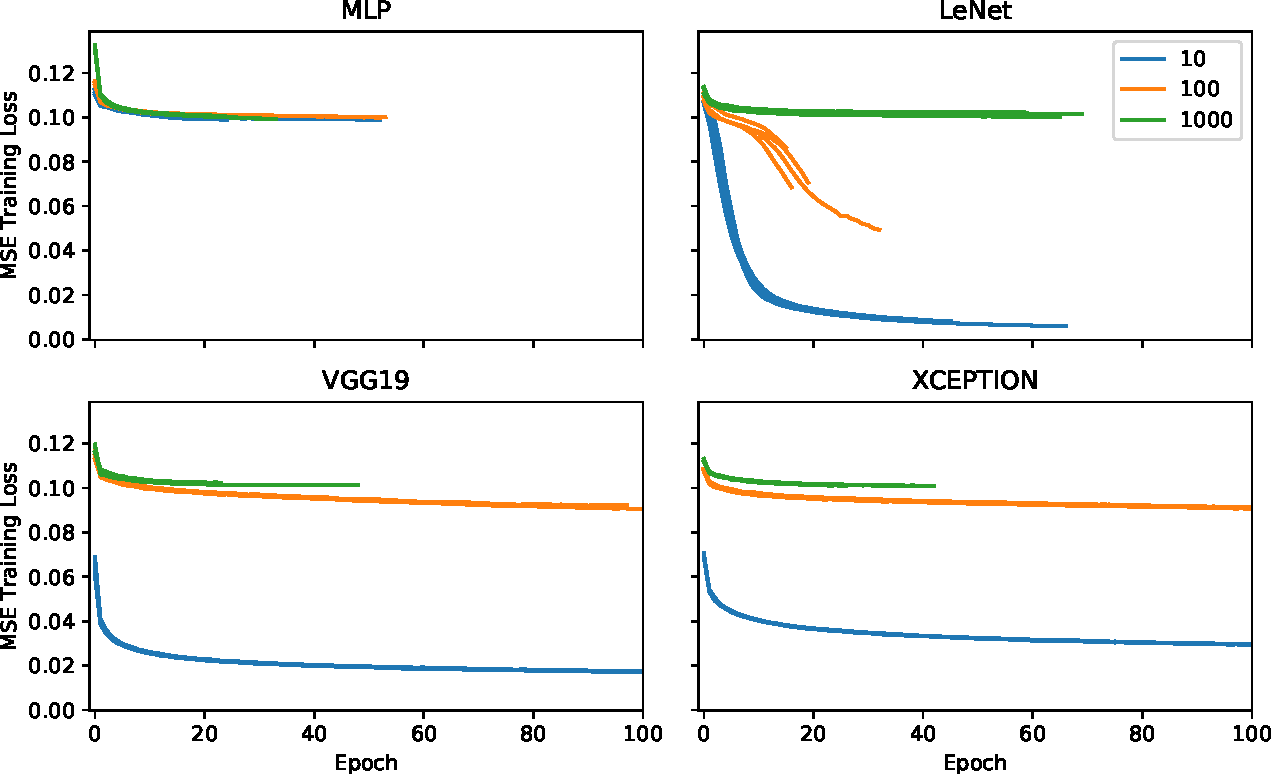
\includegraphics[width=.48\linewidth]{../gfx/weber_training_loss_no_noise.pdf}
	  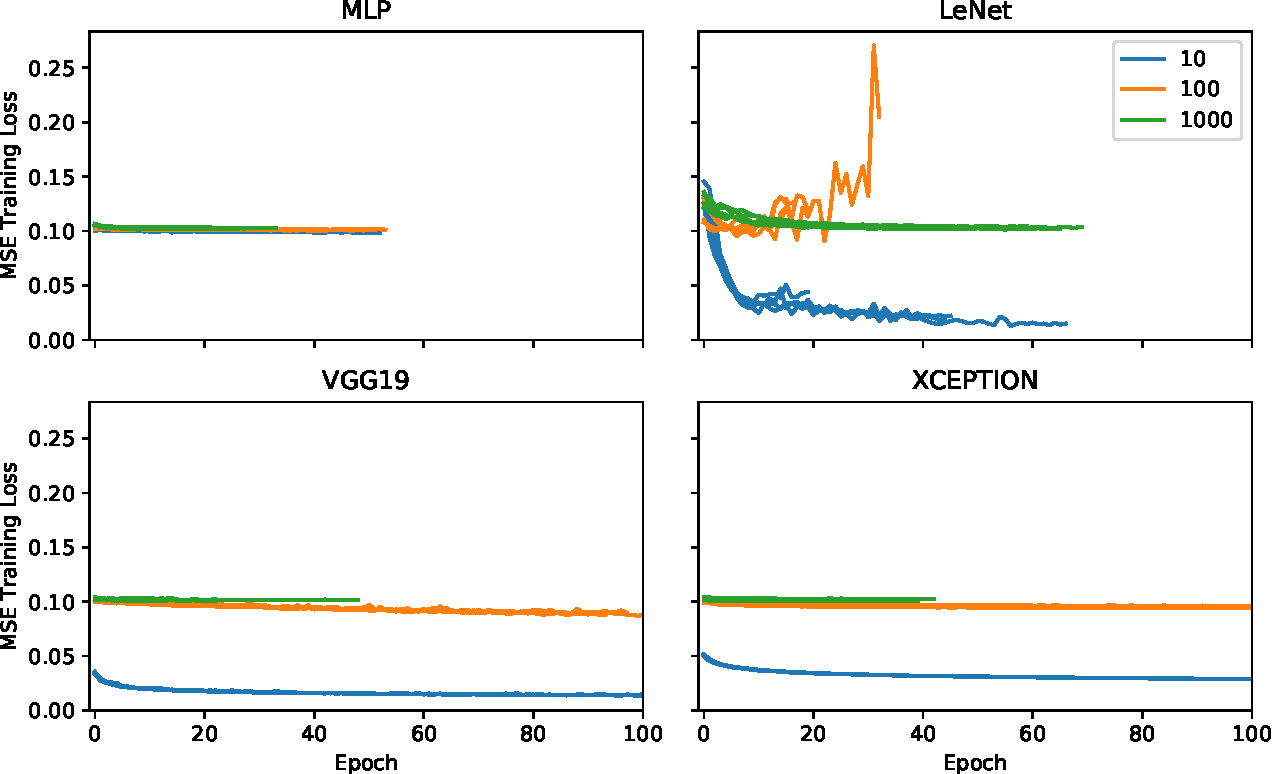
\includegraphics[width=.48\linewidth]{../gfx/weber_validation_loss_no_noise.pdf}
	}
	\hfill
    \subfloat[with noise]{
	  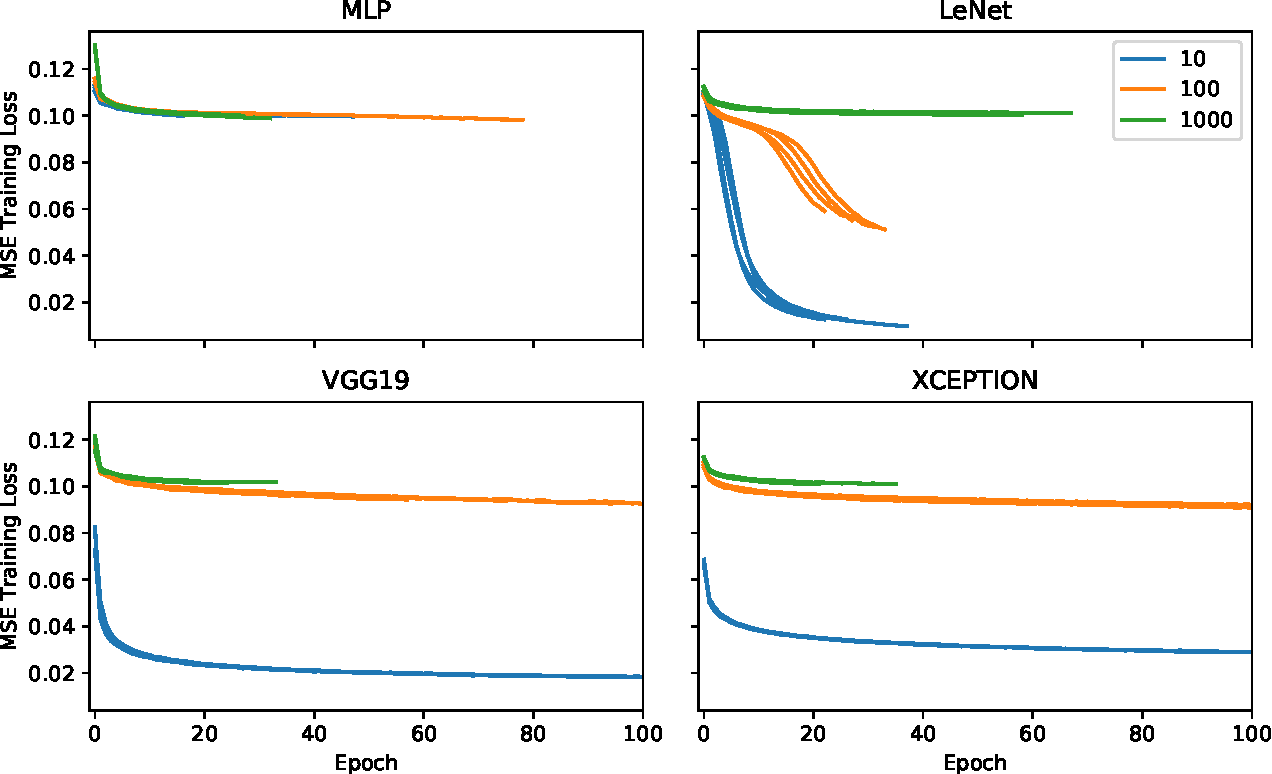
\includegraphics[width=.48\linewidth]{../gfx/weber_training_loss.pdf}
	  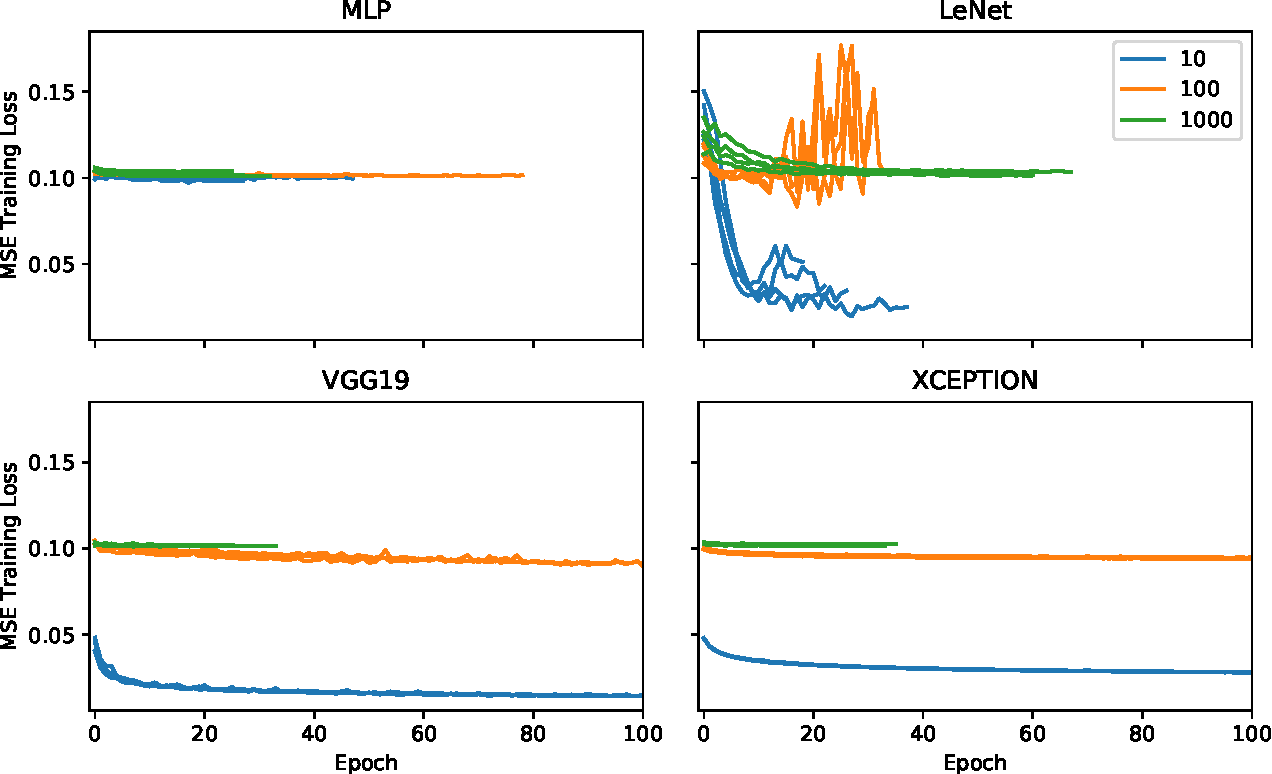
\includegraphics[width=.48\linewidth]{../gfx/weber_validation_loss.pdf}
	}

  \caption{\textbf{Loss plots for the Weber-Fechner's law experiment.} We visualize the MSE loss on training data (left) and for unseen validation data (right) after each epoch (a) without noise and (b) with subtle $5\%$ noise per pixel. There is no significant difference when noise is added. The LeNet network seems to overfit with Weber Base 100 in both cases even with dropout regularization.}
	\label{fig:weber_loss}
\end{figure*}

\begin{figure}[tbhp]
	\centering
	  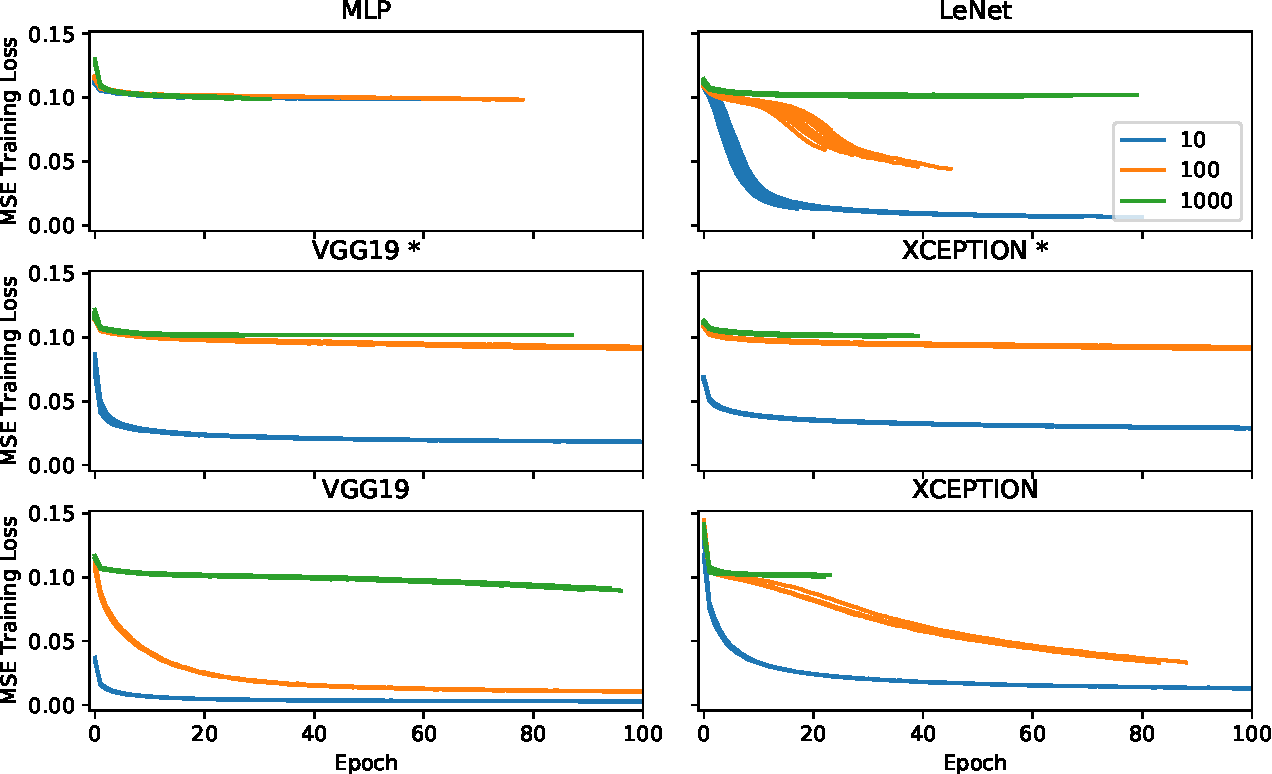
\includegraphics[width=\linewidth]{../gfx/weber_training_loss_all.pdf}
	  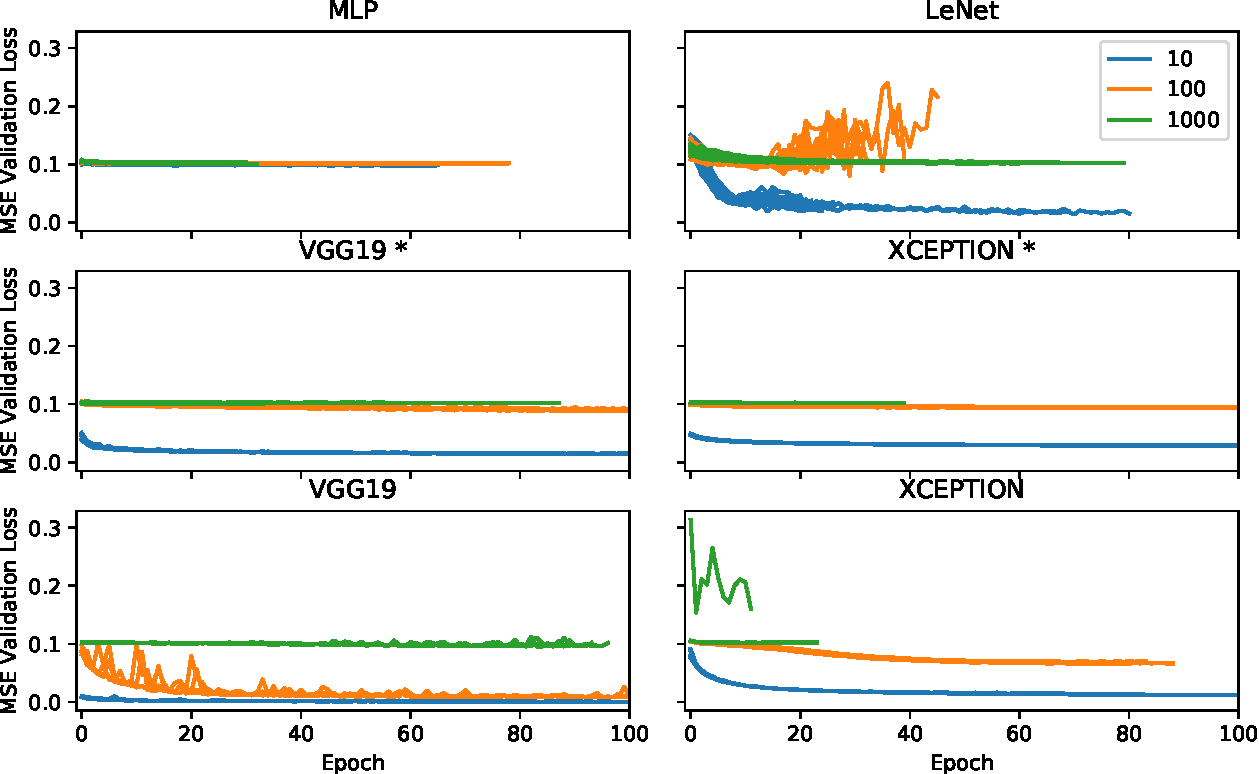
\includegraphics[width=\linewidth]{../gfx/weber_validation_loss_all.pdf}
  \caption{\textbf{Loss plots for the Weber-Fechner's law experiment including VGG19 and Xception.} We visualize the MSE loss on training data and for unseen validation data after each epoch. This plot includes the VGG19 and Xception networks trained from scratch.}
	\label{fig:weber_loss_all}
\end{figure}


\begin{figure*}[tbhp]
	\centering
	

    \subfloat[VGG19 *, Block 3 (Conv. Layers 2+3)]{
	  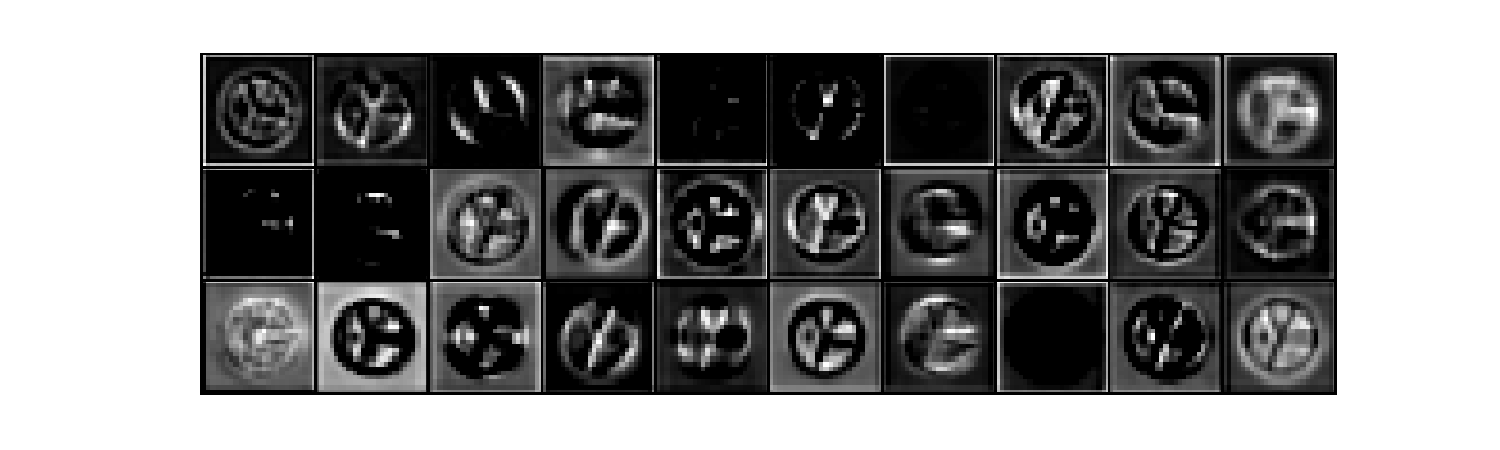
\includegraphics[width=.48\linewidth]{../gfx/ACTIVATIONMAPS/vgg_imagenet_block3_conv2.pdf}
	  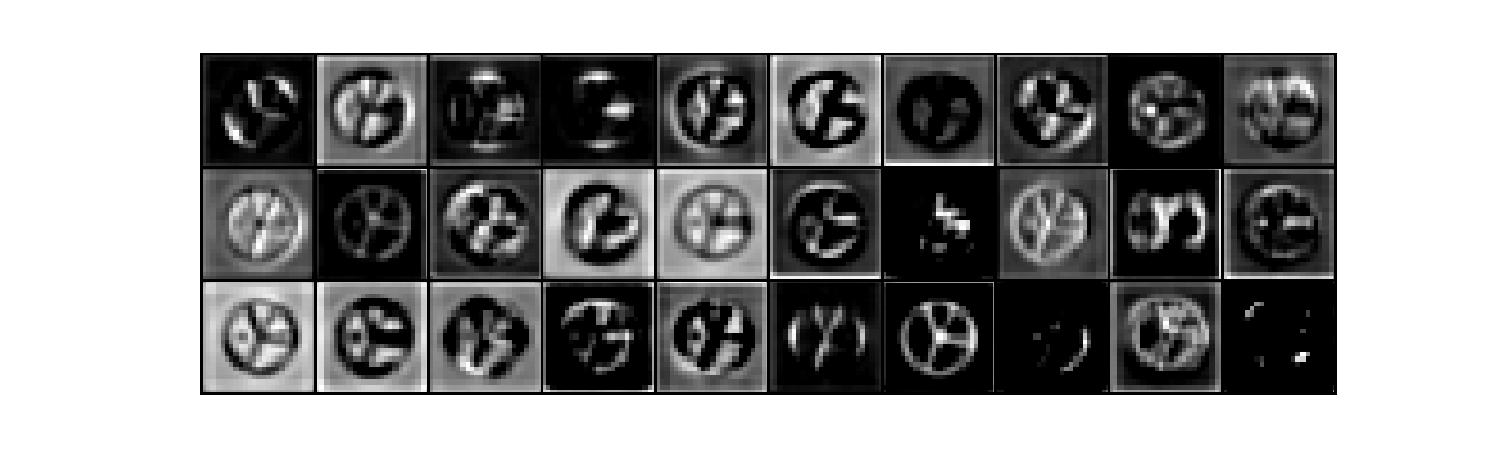
\includegraphics[width=.48\linewidth]{../gfx/ACTIVATIONMAPS/vgg_imagenet_block3_conv3.pdf}
	}
	\hfill
    \subfloat[VGG19 *, Block 4 (Conv. Layers 2+3)]{
	  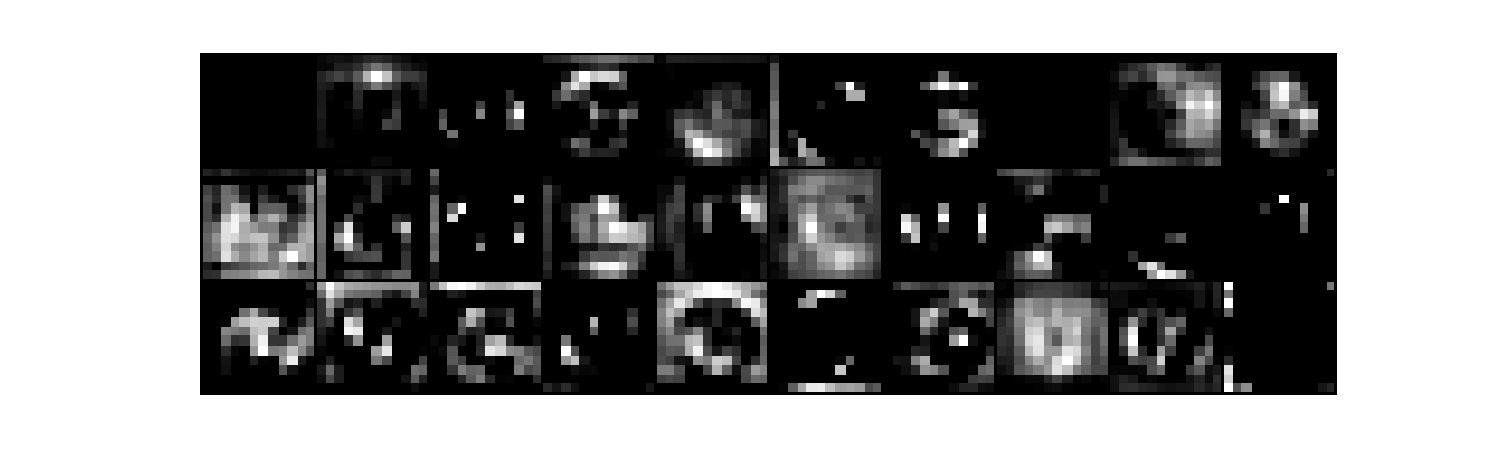
\includegraphics[width=.48\linewidth]{../gfx/ACTIVATIONMAPS/vgg_imagenet_block4_conv2.pdf}
	  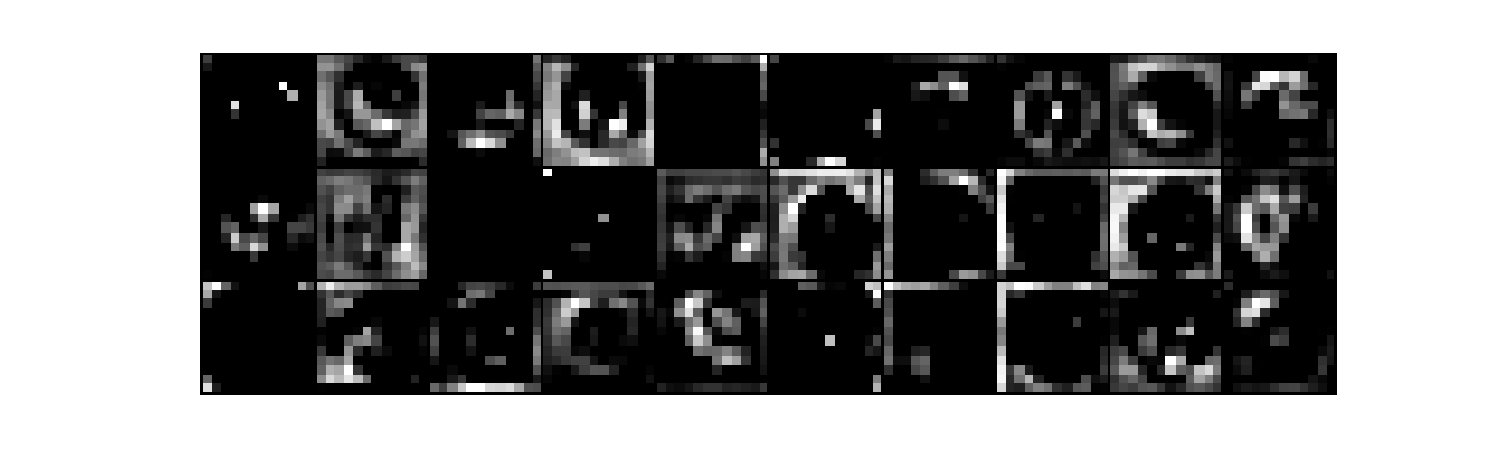
\includegraphics[width=.48\linewidth]{../gfx/ACTIVATIONMAPS/vgg_imagenet_block4_conv3.pdf}
	}
	\hfill
    \subfloat[VGG19 *, Block 5 (Conv. Layers 2+3)]{
	  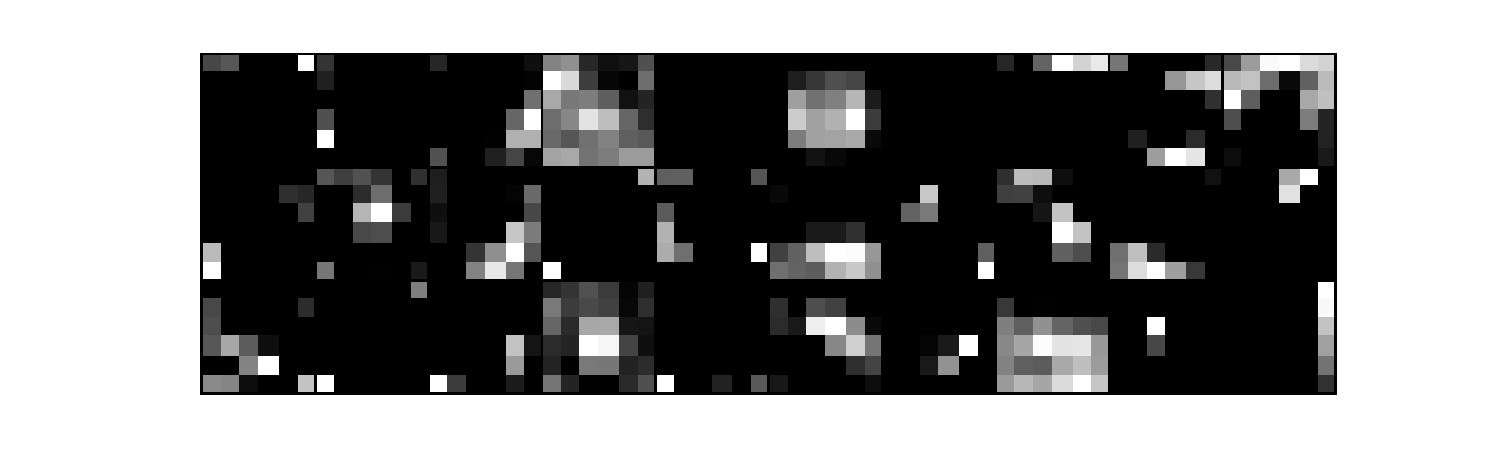
\includegraphics[width=.48\linewidth]{../gfx/ACTIVATIONMAPS/vgg_imagenet_block5_conv2.pdf}
	  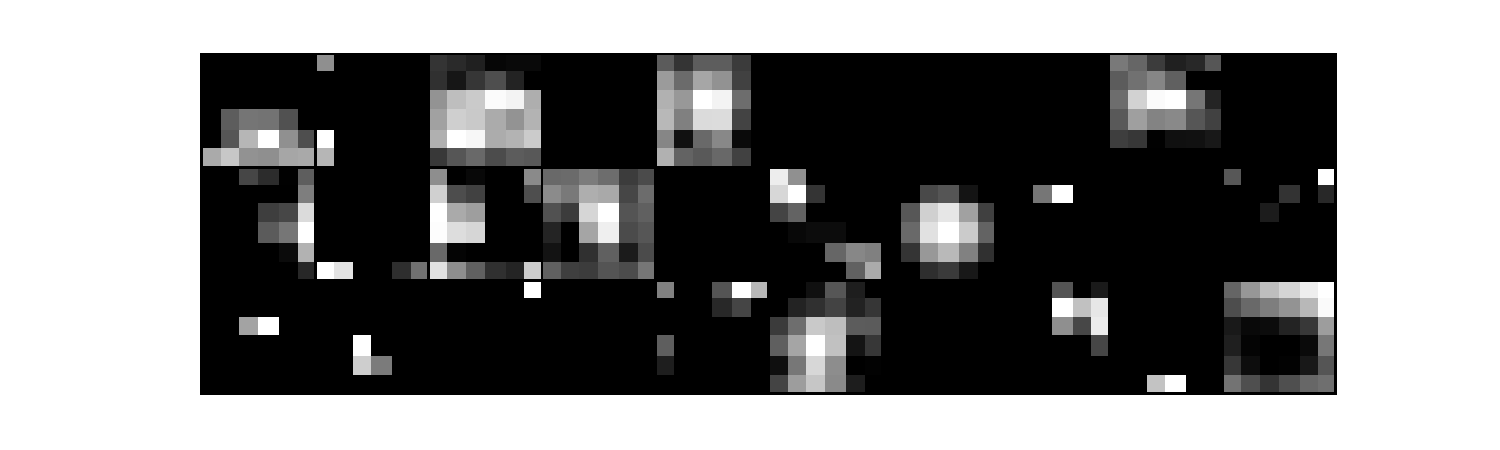
\includegraphics[width=.48\linewidth]{../gfx/ACTIVATIONMAPS/vgg_imagenet_block5_conv3.pdf}
	}
	\hfill
    \subfloat[VGG19, Block 3 (Conv. Layers 2+3)]{
	  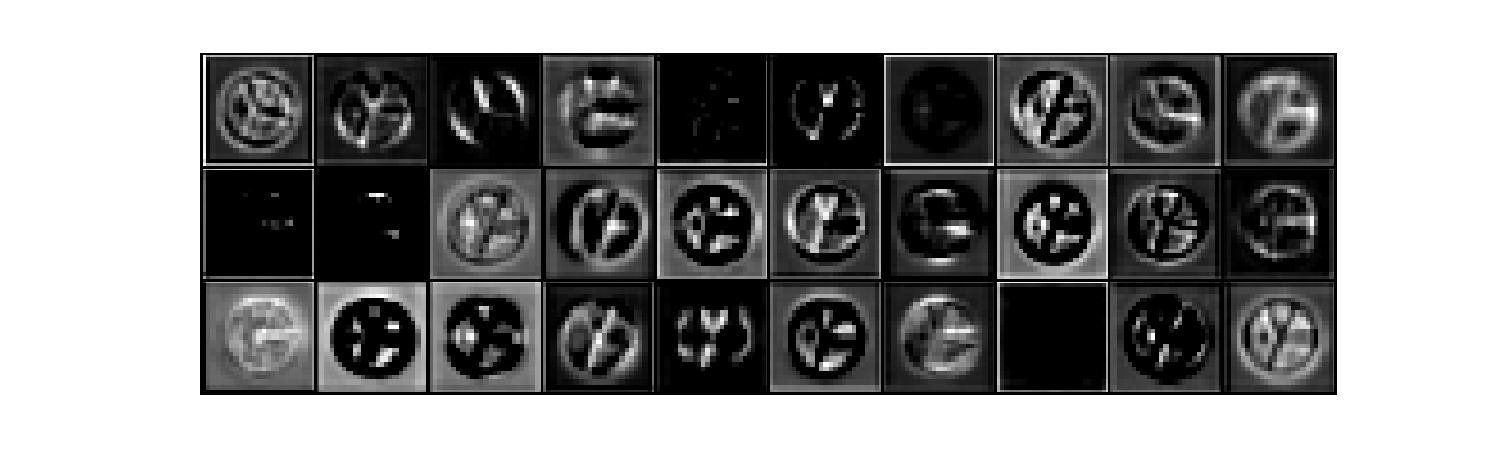
\includegraphics[width=.48\linewidth]{../gfx/ACTIVATIONMAPS/vgg_from_scratch_block3_conv2.pdf}
	  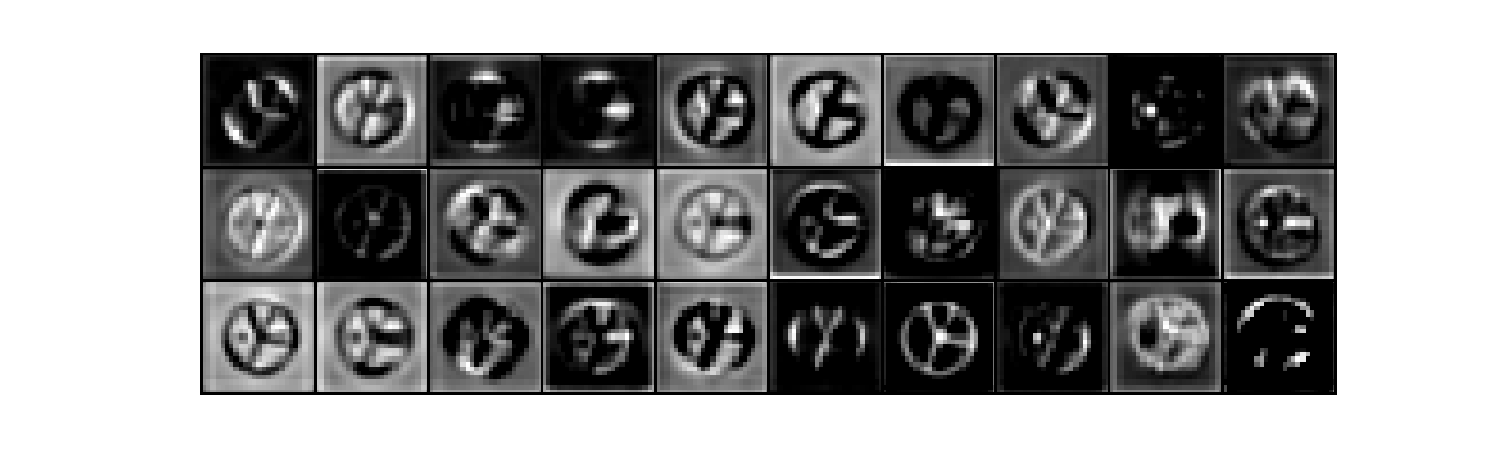
\includegraphics[width=.48\linewidth]{../gfx/ACTIVATIONMAPS/vgg_from_scratch_block3_conv3.pdf}
	}
	\hfill
    \subfloat[VGG19, Block 4 (Conv. Layers 2+3)]{
	  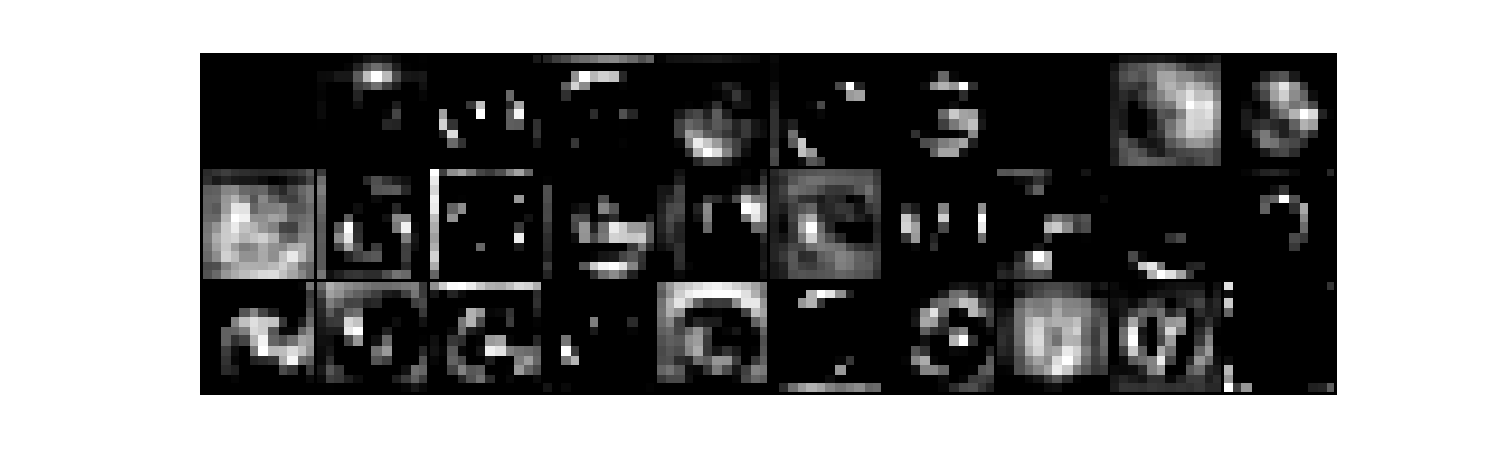
\includegraphics[width=.48\linewidth]{../gfx/ACTIVATIONMAPS/vgg_from_scratch_block4_conv2.pdf}
	  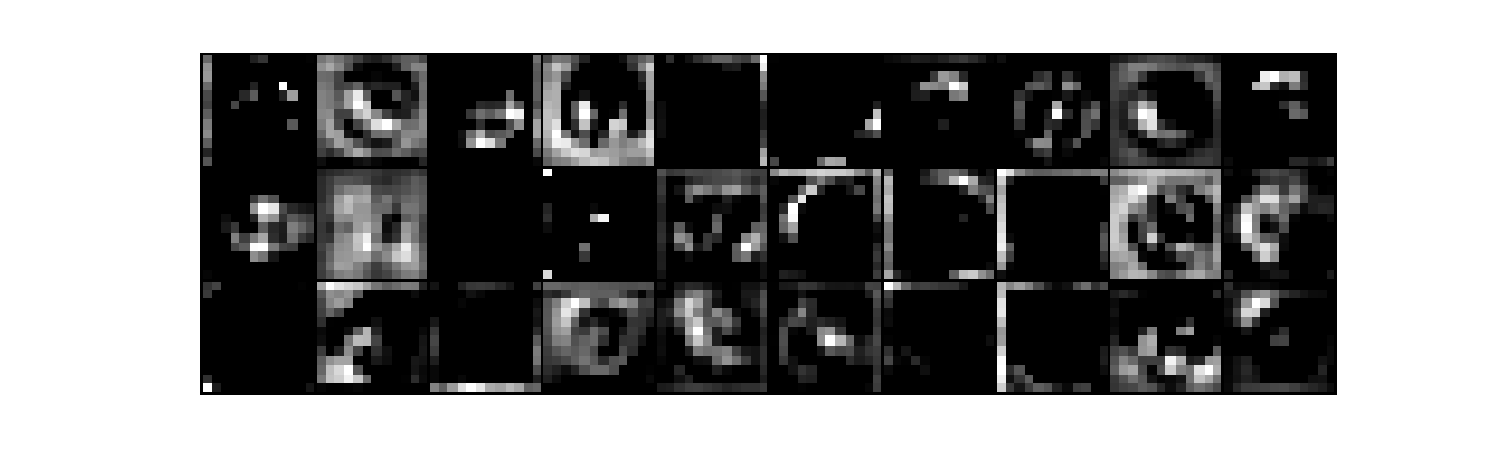
\includegraphics[width=.48\linewidth]{../gfx/ACTIVATIONMAPS/vgg_from_scratch_block4_conv3.pdf}
	}
	\hfill
    \subfloat[VGG19, Block 5 (Conv. Layers 2+3)]{
	  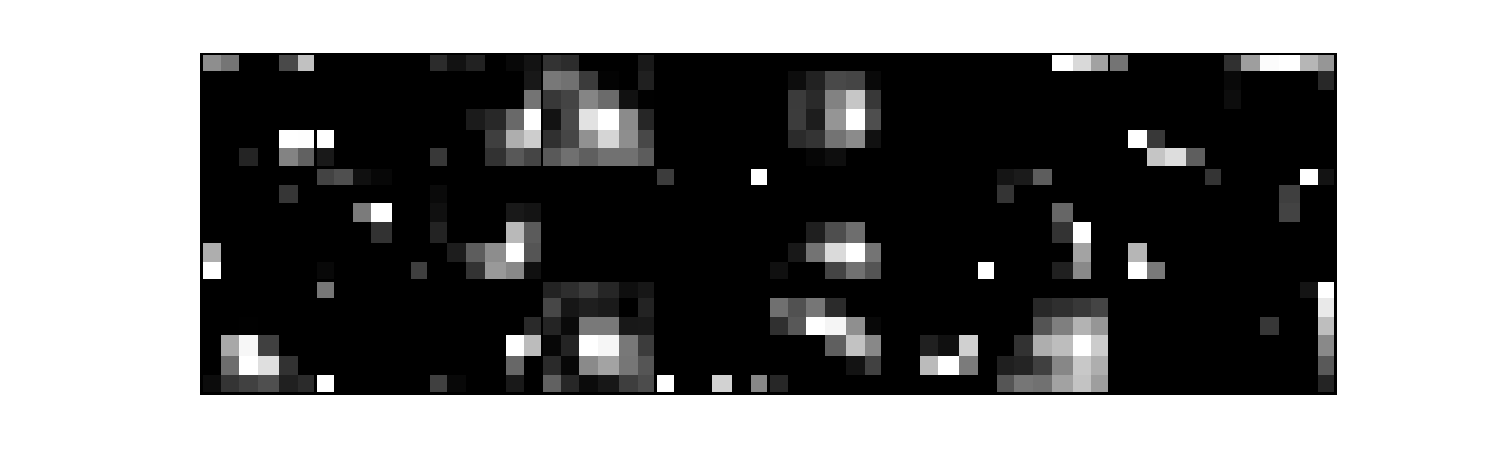
\includegraphics[width=.48\linewidth]{../gfx/ACTIVATIONMAPS/vgg_from_scratch_block5_conv2.pdf}
	  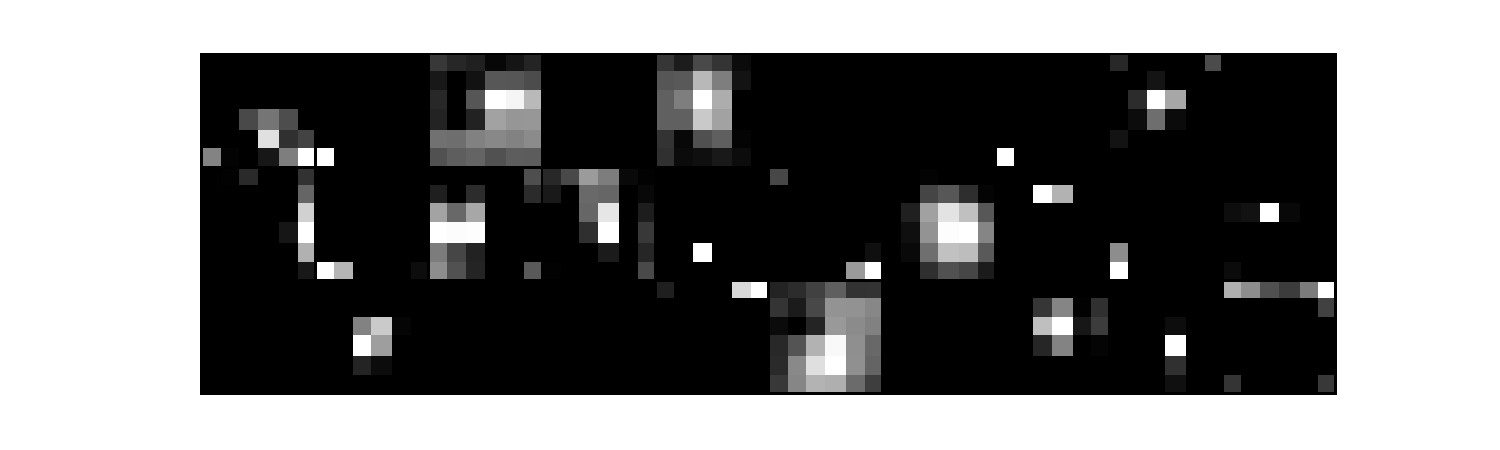
\includegraphics[width=.48\linewidth]{../gfx/ACTIVATIONMAPS/vgg_from_scratch_block5_conv3.pdf}
	}
  \caption{\textbf{Convolutional Activation Maps for a Pie Chart.} (a)-(c) is VGG19 *, trained on ImageNet. The activation maps do not differ much, which is surprising since VGG19 trained from scratch performs so much better in our experiments.}
	\label{fig:activationmaps}
\end{figure*}

\begin{figure*}[tbhp]
	\centering
	
    \subfloat[VGG19 *, Block 3 (Conv. Layers 2+3)]{
	  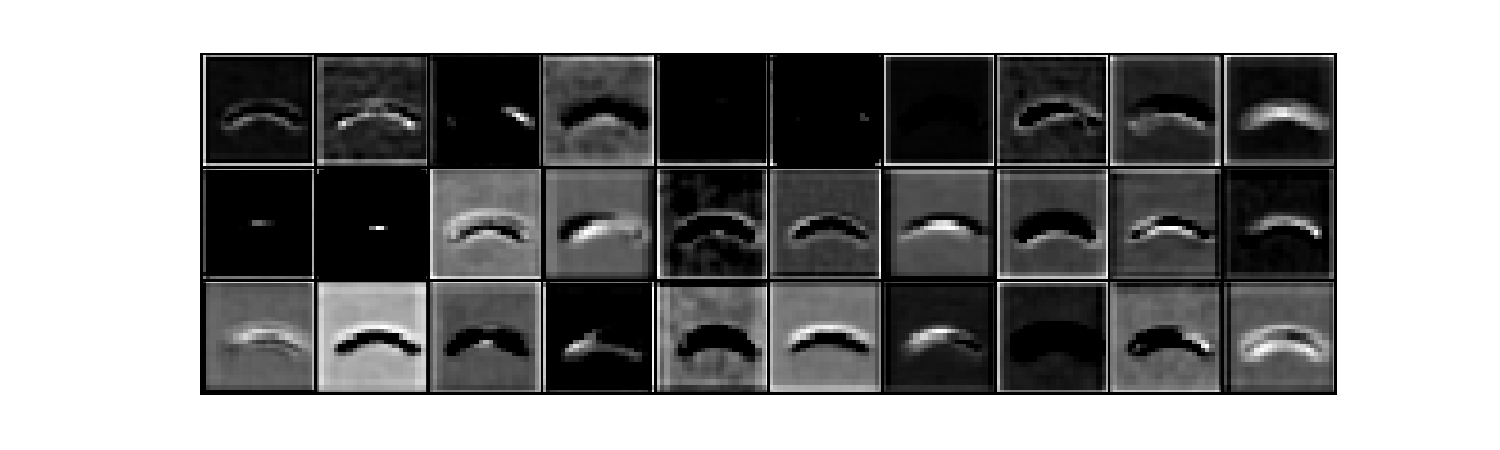
\includegraphics[width=.48\linewidth]{../gfx/ACTIVATIONMAPS/curvature_vgg_imagenet_block3_conv2.pdf}
	  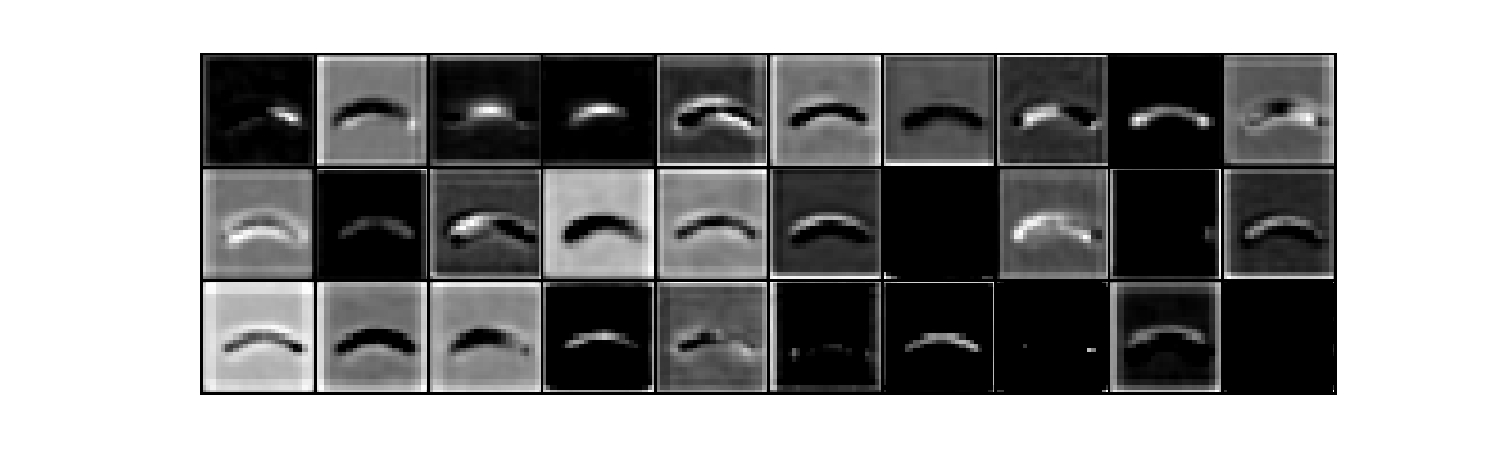
\includegraphics[width=.48\linewidth]{../gfx/ACTIVATIONMAPS/curvature_vgg_imagenet_block3_conv3.pdf}
	}
	\hfill
    \subfloat[VGG19 *, Block 4 (Conv. Layers 2+3)]{
	  \includegraphics[width=.48\linewidth]{../gfx/ACTIVATIONMAPS/curvature_vgg_imagenet_block4_conv2.pdf}
	  \includegraphics[width=.48\linewidth]{../gfx/ACTIVATIONMAPS/curvature_vgg_imagenet_block4_conv3.pdf}
	}
	\hfill
    \subfloat[VGG19 *, Block 5 (Conv. Layers 2+3)]{
	  \includegraphics[width=.48\linewidth]{../gfx/ACTIVATIONMAPS/curvature_vgg_imagenet_block5_conv2.pdf}
	  \includegraphics[width=.48\linewidth]{../gfx/ACTIVATIONMAPS/curvature_vgg_imagenet_block5_conv3.pdf}
	}
	\hfill
    \subfloat[VGG19, Block 3 (Conv. Layers 2+3)]{
	  \includegraphics[width=.48\linewidth]{../gfx/ACTIVATIONMAPS/curvature_vgg_from_scratch_block3_conv2.pdf}
	  \includegraphics[width=.48\linewidth]{../gfx/ACTIVATIONMAPS/curvature_vgg_from_scratch_block3_conv3.pdf}
	}
	\hfill
    \subfloat[VGG19, Block 4 (Conv. Layers 2+3)]{
	  \includegraphics[width=.48\linewidth]{../gfx/ACTIVATIONMAPS/curvature_vgg_from_scratch_block4_conv2.pdf}
	  \includegraphics[width=.48\linewidth]{../gfx/ACTIVATIONMAPS/curvature_vgg_from_scratch_block4_conv3.pdf}
	}
	\hfill
    \subfloat[VGG19, Block 5 (Conv. Layers 2+3)]{
	  \includegraphics[width=.48\linewidth]{../gfx/ACTIVATIONMAPS/curvature_vgg_from_scratch_block5_conv2.pdf}
	  \includegraphics[width=.48\linewidth]{../gfx/ACTIVATIONMAPS/curvature_vgg_from_scratch_block5_conv3.pdf}
	}
  \caption{\textbf{Convolutional Activation Maps for a Curvature stimuli.} (a)-(c) is VGG19 *, trained on ImageNet. The activation maps do not differ much, which is surprising since VGG19 trained from scratch performs so much better in our experiments.}
	\label{fig:activationmaps2}
\end{figure*}


\begin{figure*}[tbhp]
    \centering
	\includegraphics[width=\linewidth]{PAPER_ReviewResponse/SUPPLEMENTAL/gfx/figure12_hist.pdf}
    \caption{\change{\textbf{Bars and Framed Rectangles experiment (E4): User responses.} The responses show that users were able to precisely measure differences with the framed rectangles stimuli. For bars, the estimations were often guessed as 10 ($N=55$).}}
\end{figure*}

\begin{figure*}[tbhp]
	\includegraphics[width=\linewidth]{PAPER_ReviewResponse/SUPPLEMENTAL/gfx/weber_hist.pdf}
    \caption{\change{\textbf{Weber's law point cloud experiment (E5): User responses.} The human results for 10, 100, 1,000 points exhibit skewed distributions. At 1,000 points, this task is virtually impossible, and so humans resort to simply guessing. However, they seem to `guess high', leading to worse than random performance on the task.}}
\end{figure*}



\clearpage
\begin{table*}[tbhp]

\caption{\change{Mean squared error (MSE) for the elementary perceptual tasks experiment (E1), to accompany the midmean logistic absolute error metric (MLAE) measures in the main paper.}}

\resizebox{\linewidth}{!}{
\begin{tabular}{lrrrrrr}
\toprule
  & MLP & LeNet & VGG19 * & VGG19 & Xception * & Xception \\
\midrule
Position Common Scale & $0.03794 \pm 0.01436 $ & $0.00106 \pm 0.00028 $ & $0.00079 \pm 0.00027 $ & $0.00014 \pm 0.00009 $ & $0.00170 \pm 0.00036 $ & $0.00074 \pm 0.00034 $   \\ 
Position Non-aligned Scale & $0.02974 \pm 0.00912 $ & $0.00097 \pm 0.00043 $ & $0.00081 \pm 0.00016 $ & $0.00021 \pm 0.00013 $ & $0.00183 \pm 0.00047 $ & $0.00060 \pm 0.00006 $   \\ 
Length & $0.00267 \pm 0.00053 $ & $0.01044 \pm 0.00301 $ & $0.00046 \pm 0.00050 $ & $0.00010 \pm 0.00002 $ & $0.00142 \pm 0.00021 $ & $0.00066 \pm 0.00010 $   \\ 
Direction & $0.08359 \pm 0.00645 $ & $0.01409 \pm 0.00575 $ & $0.01014 \pm 0.00212 $ & $0.00121 \pm 0.00090 $ & $0.02342 \pm 0.00556 $ & $0.00247 \pm 0.00159 $   \\ 
Angle & $0.08092 \pm 0.00953 $ & $0.01859 \pm 0.00611 $ & $0.00415 \pm 0.00087 $ & $0.00053 \pm 0.00006 $ & $0.00607 \pm 0.00064 $ & $0.00158 \pm 0.00019 $   \\ 
Area & $0.00256 \pm 0.00074 $ & $0.00383 \pm 0.00171 $ & $0.00031 \pm 0.00016 $ & $0.00010 \pm 0.00004 $ & $0.00047 \pm 0.00013 $ & $0.13955 \pm 0.22880 $   \\ 
Volume & $0.00593 \pm 0.00382 $ & $0.00405 \pm 0.00567 $ & $0.00100 \pm 0.00067 $ & $0.00084 \pm 0.00065 $ & $0.00339 \pm 0.00218 $ & $0.00346 \pm 0.00050 $   \\ 
Curvature & $0.00343 \pm 0.00076 $ & $0.00065 \pm 0.00015 $ & $0.00024 \pm 0.00003 $ & $0.00006 \pm 0.00001 $ & $0.00047 \pm 0.00010 $ & $0.00254 \pm 0.00108 $   \\ 
Shading & $0.01861 \pm 0.00811 $ & $0.00448 \pm 0.00205 $ & $0.00078 \pm 0.00067 $ & $0.00032 \pm 0.00021 $ & $0.00303 \pm 0.00138 $ & $0.00657 \pm 0.00473 $   \\ 
\bottomrule
\end{tabular}
}
\end{table*}


\begin{table*}[tbhp]

\caption{\change{Mean squared error (MSE) for the position-angle experiment (E2), to accompany the midmean logistic absolute error metric (MLAE) measures in the main paper}}

\resizebox{\linewidth}{!}{
\begin{tabular}{lrrrrrr}
\toprule
  & MLP & LeNet & VGG19 * & VGG19 & Xception * & Xception \\
\midrule
Pie Chart & $0.04725 \pm 0.00177 $ & $0.02429 \pm 0.00070 $ & $0.02492 \pm 0.00143 $ & $0.00095 \pm 0.00018 $ & $0.01371 \pm 0.00078 $ & $0.00260 \pm 0.00037 $  \\ 
Bar Chart & $0.00629 \pm 0.00051 $ & $0.00322 \pm 0.00029 $ & $0.00723 \pm 0.00107 $ & $0.00076 \pm 0.00012 $ & $0.00465 \pm 0.00020 $ & $0.00109 \pm 0.0001 $  \\ 
\bottomrule
\end{tabular}
}
\end{table*}


\begin{table*}[tbhp]

\caption{\change{Mean squared error (MSE) for the position-length experiment (E3), to accompany the midmean logistic absolute error metric (MLAE) measures in the main paper.}}

\resizebox{\linewidth}{!}{
\begin{tabular}{lrrrrrr}
\toprule
  & MLP & LeNet & VGG19 * & VGG19 & Xception * & Xception \\
\midrule
Type 1 & $0.03561 \pm 0.01403 $ & $0.13262 \pm 0.07927 $ & $0.04563 \pm 0.02225 $ & $0.04259 \pm 0.01621 $ & $0.07448 \pm 0.04100 $ & $0.10515 \pm 0.04370 $   \\ 
Type 2 & $0.04270 \pm 0.04115 $ & $0.07342 \pm 0.04200 $ & $0.12256 \pm 0.06932 $ & $0.03976 \pm 0.02488 $ & $0.04624 \pm 0.02606 $ & $0.08235 \pm 0.02587 $   \\ 
Type 3 & $0.06055 \pm 0.02853 $ & $0.04998 \pm 0.08381 $ & $0.09711 \pm 0.04050 $ & $0.02746 \pm 0.01733 $ & $0.03701 \pm 0.01777 $ & $0.08443 \pm 0.04828 $   \\ 
Type 4 & $0.07275 \pm 0.03090 $ & $0.05433 \pm 0.04709 $ & $0.03922 \pm 0.02143 $ & $0.03065 \pm 0.02038 $ & $0.05543 \pm 0.06636 $ & $0.06119 \pm 0.06254 $   \\ 
Type 5 & $0.06728 \pm 0.02543 $ & $0.03583 \pm 0.02154 $ & $0.12193 \pm 0.05223 $ & $0.04314 \pm 0.03622 $ & $0.04574 \pm 0.01683 $ & $0.07167 \pm 0.02072 $   \\ 
Multi & $0.02624 \pm 0.01729 $ & $0.04419 \pm 0.02724 $ & $0.07631 \pm 0.02532 $ & $0.01756 \pm 0.00931 $ & $0.03850 \pm 0.02710 $ & $0.08365 \pm 0.02061 $   \\ 
\bottomrule
\end{tabular}
}
\end{table*}


\begin{table*}[tbhp]

\caption{\change{Mean squared error (MSE) for the bars and framed rectangles experiment (E4), to accompany the midmean logistic absolute error metric (MLAE) measures in the main paper}}

\resizebox{\linewidth}{!}{
\begin{tabular}{lrrrrrr}
\toprule
  & MLP & LeNet & VGG19 * & VGG19 & Xception * & Xception \\
\midrule
Framed Rectangles & $0.00065 \pm 0.00012 $ & $0.01343 \pm 0.00484 $ & $0.00156 \pm 0.00029 $ & $0.00032 \pm 0.00011 $ & $0.00437 \pm 0.00069 $ & $0.00155 \pm 0.00062 $   \\ 
Bars & $0.00060 \pm 0.00012 $ & $0.00553 \pm 0.00196 $ & $0.00173 \pm 0.00037 $ & $0.00043 \pm 0.00024 $ & $0.00531 \pm 0.00073 $ & $0.00145 \pm 0.00053 $   \\ 
\bottomrule
\end{tabular}
}
\end{table*}


\begin{table*}[tbhp]

\caption{\change{Mean squared error (MSE) for the Weber's law point cloud experiment (E5), to accompany the midmean logistic absolute error metric (MLAE) measures in the main paper.}}

\resizebox{\linewidth}{!}{
\begin{tabular}{lrrrrrr}
\toprule
  & MLP & LeNet & VGG19 * & VGG19 & Xception * & Xception \\
\midrule
10 points  & $0.10126 \pm 0.00062 $ & $0.13759 \pm 0.03183 $ & $0.09031 \pm 0.00130 $ & $0.00899 \pm 0.00150 $ & $0.09354 \pm 0.00078 $ & $0.06830 \pm 0.00207 $   \\ 
100 points & $0.10250 \pm 0.00057 $ & $0.10259 \pm 0.00065 $ & $0.10202 \pm 0.00038 $ & $0.09835 \pm 0.00267 $ & $0.10174 \pm 0.00034 $ & $0.10818 \pm 0.01003 $   \\ 
1,000 points & $0.09946 \pm 0.00095 $ & $0.03436 \pm 0.01137 $ & $0.01477 \pm 0.00059 $ & $0.00076 \pm 0.00008 $ & $0.02610 \pm 0.00026 $ & $0.01041 \pm 0.00258 $   \\
\bottomrule
\end{tabular}
}
\end{table*}

%% if specified like this the section will be committed in review mode
%\acknowledgments{
%The authors wish to thank A, B, and C. This work was supported in part by
%a grant from XYZ (\# 12345-67890).}

\end{document}

